\documentclass{article}
\usepackage[utf8]{inputenc}
\usepackage{amsmath}
\usepackage{amssymb}
\usepackage{titlesec}
\newcommand{\sectionbreak}{\clearpage}
\usepackage{hyperref}
\usepackage{amsthm}
\usepackage{stmaryrd}
\usepackage{mathtools}

\usepackage{tikz}

\setlength{\parindent}{0pt}
\setlength{\parskip}{0.5em}

\theoremstyle{definition}
\newtheorem{defn}{Definition}[section]
\newtheorem{conj}{Conjecture}[section]
\newtheorem{exmp}{Example}[section]

\theoremstyle{plain}% default
\newtheorem{thm}{Theorem}[section]
\newtheorem{lem}[thm]{Lemma}
\newtheorem{prop}[thm]{Proposition}
\newtheorem*{cor}{Corollary}
\newtheorem*{clm}{Claim}

\theoremstyle{remark}
\newtheorem*{rem}{Remark}
\newtheorem*{note}{Note}
\newtheorem*{rec}{Recall}

\newcommand{\R}{\mathbb{R}}
\newcommand{\Q}{\mathbb{Q}}
\newcommand{\C}{\mathbb{C}}
\newcommand{\Z}{\mathbb{Z}}
\newcommand{\F}{\mathbb{F}}
\newcommand{\Emb}{\text{Emb}}
\newcommand{\Gal}{\text{Gal}}
\newcommand{\Out}{\text{Out}}


\newcommand{\onetoone}{\stackrel{\mathclap{\normalfont\mbox{1to1}}}{\;=\;}}

\title{Galois Theory Notes}
\author{Emma}
\date{Spring 2019}

\begin{document}

\maketitle

\tableofcontents

\section{Fundamental Theorem of Galois Theory}

\begin{thm}[\textbf{Fundamental Theorem of Galois Theory}]
Assume characteristic 0. Let $k \subset L$ and $L$ is the splitting field of $f(x) \in k[X]$. Let \[G = \{\sigma : L \to L\ | \; \sigma \text{ is a field outermorphism of } L \text{ with } \sigma_{|k} = id_k\}\] we call this the Galois group. \\
There is a 1-to-1 correspondence: \[\{k \subset K \subset L\} \longleftrightarrow \{H \le G, H \text{ a subgroup}\}\]
\[K \mapsto \{\sigma \in G \; | \; \forall \lambda \in K, \sigma(\lambda) = \lambda\}\] \[\{\lambda \in L \; | \; \forall \sigma \in H, \sigma(\lambda) = \lambda\} \mapsfrom H \le G \]
In other words, we have the mapping
\begin{itemize}
    \item $k \subset K \subset L$ maps to the group of automporphisms of $L$ which fix all of $K$ as well as $k$
    \item $H < G$ is a group of automorphisms of $L$, which maps to the field that all those automorphisms fix (which is always an extension of $k$)
\end{itemize}
\end{thm}



\begin{rem}
We use this to study fields, as fields are "hard" and groups are "easy". We will see that there is a good formula for the roots of $f(x)$ if and only if $G$ the Galois group is a soluble group.
\end{rem}

\begin{exmp}
Assume $K$ does not have characteristic 2. Let $L$ be the splitting field for $K$ with $f$ having degree 2, i.e. $f(x) = x^2 + 2Ax + B \in K[X]$.

If $K$ already contains the roots of the polynomial, then $L = K$ and $G = \{\text{id}\}$.

If $K$ doesn't contain the roots of the polynomial, then we can use the quadratic formula: \[\lambda_{1,2} = -A \pm \sqrt{A^2 - B}\]
If $\delta = A^2 - B$, then $\sqrt{\delta}$ does not exists in $K$. We must have therefore $L = K(\sqrt{\delta}) = \{a + b\sqrt{\delta} \; | \; a,b \in K\}$.

We have that the Galois group is the cyclic group of order 2, $C_2$. The Galois group is the group of automorphisms $\sigma : L \to L$, where for every $k \in L \subset K$, we have that $\sigma(k) = k$. So the only values $\sigma$ can change are the values generated by the roots of the polynomial $f$ (in this case, the values generated by $\sqrt{\delta}$. We can check that $\sigma(\sqrt{\delta}) = -\sqrt{\delta}$ is an automorphism, and that it is the only automorphism other than the identity map, which has order 2 ($\sigma^2(\sqrt{\delta}) = \sqrt{\delta}$. Hence, the group is isomorphic to the cyclic group of order 2. 
\end{exmp}

We can specialise this further
\begin{exmp}
\item Let $K = \R, \delta = -1$. Then
\[ L = \{ a + b\sqrt{-1} | a, b \in \R\}\]
and as we stated before, $G$ is isomorphic to $C_2$, so there are two elements, and they both must preserve the integers. Thus we have
\[G = \{ \text{id}, a + b\sqrt{-1} \mapsto a - b\sqrt{-1} \}\]
\end{exmp}

\begin{exmp}[Cubic extension]
Take $f(X) = X^3 - 2$ in $\Q[X]$. Then the splitting field of $f(X)$ is $L = \Q(\sqrt[3]{-2}, \omega)$ where $\omega = \frac{-1 + i\sqrt{3}}{2}$ - and 
\[f(X) = (X - \sqrt[3]{-2})(X - \omega\sqrt[3]{-2})(X - \omega^2\sqrt[3]{-2})\]
and we immediately find that there are many different subfields of $L$ -
\[\Q(\sqrt[3]{-2}), \Q(\omega\sqrt[3]{-2}), \Q(\omega^2\sqrt[3]{-2}), \Q(\omega)\]
and we can investigate other combinations, such as $\Q(\sqrt[3]{-2} + \omega)$ and $\Q(\sqrt[3]{-2}, \omega\sqrt[3]{-2})$, and ask if these are proper subfields of $L$ or not. In fact, there are no other subfields (this is left as an exercise).
\end{exmp}

\begin{prop}[Inclusion of Galois group in $S_n$]\label{Galois incl prop}
For a polynomial $f(X) = X^n + a_1X^{n-1} + \dots + a_n \in K[X]$, there is \underline{always} an inclusion homomorphism $\rho$ from the Galois group $G$ to the permutation group ($S$) of the roots of the polynomial in the splitting field $L$ - this permutation group is $S(\lambda_1, \lambda_2, \dots, \lambda_n)$.
\end{prop}

\begin{proof}
Take any $\sigma \in G$ the Galois group. Then we have that \[f(\lambda_i) = 0 = \sigma(0) = \sigma(f(\lambda_i)))\] \[\sigma(\lambda_i^n + a_1\lambda_i^{n-1} + ... + a_n) = 0\] and as $\sigma$ fixes $K$, \[\sigma(\lambda_i)^n + a_1\sigma(\lambda_i)^{n-1} + .. + a_n = 0\] Hence we must have that for all $\lambda_i$, $\sigma(\lambda_i)$ is also a root of $f(X)$. This means that all $\sigma \in G$ are permutations of the roots $\lambda_i$ of $f(X)$, hence $G \subseteq S(\lambda_i)$ (the permutation group of the roots).
\end{proof}



\section{Field Theory Background}

\subsection{Background}

\begin{defn}[Field homomorphisms]
A field homomorphism is a function $\phi: K_1 \to K_2$ that preserves field operations: \[\phi(0_{K_1}) = 0_{K_2}\] \[\phi(1_{K_1}) = 1_{K_2}\] \[\phi(a+b) = \phi(a) + \phi(b) \] \[\phi(ab) = \phi(a)\phi(b)\]
\end{defn}

\begin{rem}
All field homomorphisms are injective.
\end{rem}

\begin{proof}
If $a \in K_1 / \{0\}$ then $\exists b \in K_1$ such that $ab = 1$. Using the homomorphism definition, we have $\phi(a)\phi(b) = 1$ hence $\phi(a) \ne 0$. This easily implies $\phi$ is injective: take $a_1 \ne a_2$, then $a_1 - a_2 \ne 0$ so $\phi(a_1 - a_2) = \phi(a_1) - \phi(a_2) \ne 0$ hence $\phi(a_1) \ne \phi(a_2)$.
\end{proof}

\begin{flushleft}
Galois theory concerns itself with field extensions (namely algebraic ones).
\end{flushleft}

\begin{rec}
The \textit{smallest} field extension of a field $K$ containing a value $\alpha \not\in K$ is $K(\alpha)$.
\end{rec}

\begin{exmp}
Take $\mathbb{Q} \subset \mathbb{C}$. We can extend $\mathbb{Q}$ by $\alpha = \sqrt{2}$ or $\alpha{\pi}$.
\end{exmp}

\begin{rec}
$\alpha$ is algebraic in $K$ if there exists an $f(X) \in K[X]$ such that $f(\alpha) = 0$. Otherwise $\alpha$ is transcendental. We say $k$ is algebraic in $K$ if $\forall \alpha \in K$, we have that $\alpha$ is algebraic in $k$ ($k$ is just algebraic if it is algebraic in its field of fractions).
\end{rec}

\begin{defn}[Splitting fields]
Take fields $K \subset L$. We say that $L$ is a splitting field for $f$ if: \[f(X) = a\prod_{i=1}^n(X - \lambda_i) \in L[X]\] \[L = K(\lambda_1, \lambda_2, .., \lambda_n)\]
i.e. take a function $f$ in $K[X]$, factor it into roots (that may be in $K$) and extend $K$ by those roots - the resulting field extension is called a splitting field for that function $f$.
\end{defn}

\begin{exmp}
Let $f(x) = x^2 - 2 \in \mathbb{Q}[X]$. The $K = \mathbb{Q}(\sqrt{2})$ is a splitting field for $f$. Indeed, $f(x) = x^2 - 2 = (x - \sqrt{2})(x + \sqrt{2}) \in \mathbb{Q}(\sqrt{2})[X]$. 
\end{exmp}

\begin{exmp}
Let $f(x) = x^3 - 2 \in \mathbb{Q}[X]$. Then $\mathbb{Q}(\sqrt[3](2))$ is \textbf{NOT} a splitting field for $f$: $f(x) = x^3 - 2 = (x - \sqrt[3](2))(x - \omega \sqrt[3](2))(x - \omega^2 \sqrt[3](2))$ where $\omega = \frac{-1 + \sqrt{-3}}{2} \not\in \mathbb{Q}(\sqrt[3](2))$.
\end{exmp}

\begin{prop}[Tower law of finite extensions]
If we have $K \subset L \subset F$ are all finite extensions of fields, then $[F:K] = [F:L][L:K]$.
\end{prop}

\begin{lem}
Suppose $y_1, ..., y_n \in F$ is a basis of $F$ as a vector space over $L$, ad suppose $x_1, .., x_m \in L$ is a basis of $L$ as a vector space. Then $\{x_i, y_j\}$ is a basis of $F$ over $K$.
\end{lem}

\begin{proof}
Let $z \in F$. Then $\exists \mu_1, .. \mu_n \in L$ such that $z = \mu_1y_1 + .. + \mu_ny_n$, but $\mu_j \in L$ so $\forall j \exists \lambda_{ij} \in K$ such that $\mu_j = x_1\lambda_1 + ... + x_n\lambda_{mj}$.
So every $z$ in $F$ can be written as $\sum_{i,j} \lambda_{ij}x_iy_j$.

The $\{x_i,y_j\}$ are also linearly independent. Since the $y_j$s are in $F$, we cannot generate them by any $x_i$, and they are linearly independent themselves, but $x_i$s are also linearly independent so the coefficients $\lambda_{ij}$ must be zero for their sum to be zero.
\end{proof}

\begin{proof}
Use the lemma.
\end{proof}

\subsection{Example: $\Q(\sqrt[3]{2}, \omega)$}

Taking $L = \Q(\sqrt[3]{2}, \omega)$ to be the splitting field of $x^3 - 2$, we can list the subfields as $\Q, \Q(\sqrt[3]{2}), \Q(\omega), \Q(\omega\sqrt[3]{2}), \Q(\omega^2\sqrt[3]{2}), \Q(\sqrt[3]{2}, \omega)$.

\begin{clm}
There are no other sub-fields.
\end{clm}

\begin{defn}
$K \subset L$ is finite  if $L$ is finite dimensional as a vector space over $K$. Then we say $\text{degree}_K L = [L:K] = dim_K L$.
\end{defn}

\begin{prop}\label{Poly ext prop}[Extension of polynomial roots]
Suppose $f(x) \in K[X]$ is an irreducible polynomial of degree $d$, and that $L = K(\lambda)$ where $\lambda$ is a root of $f$. Then the degree of the extension $[K(\lambda) : K] = d$.
\end{prop}

\begin{exmp}
Let $f(x) = x^3 - 2$. Let $\lambda = \sqrt[3]{2}$ be a root of $f$. Then \\ $[\Q(\sqrt[3]{2}) : \Q] = 3$: we can see this as $\Q(\sqrt[3]{2}) = \{a + b\sqrt[3]{2} + c\sqrt[3]{4} \; | \; a,b,c \in \Q\}$ which is a vector in 3 dimensions over the field $\Q$.
\end{exmp}

Using the tower law, we can find the dimensions of the subfields over $\Q$ we currently have: $\Q : 1, \Q(\sqrt[3]{2}) : 3, \Q(\omega) : 2, \Q(\omega\sqrt[3]{2}) : 3, \Q(\omega^2\sqrt[3]{2}) : 3, \Q(\sqrt[3]{2}, \omega) : 6$. Any other field must have dimension either $2,3$ over $\Q$.

Suppose $[K : \Q] = 2$. Either $\omega \in K$ i.e. $\Q(\omega) \subseteq K$ and hence by the tower law $K = \Q(\omega)$, or $\omega \not\in K$ hence $x^2 + x + 1 \in K[X]$ is irreducible so $[K(\omega) : K] = 2$ therefore $[K(\omega) : \Q] = 4$, which contradicts the tower law.

Suppose $[K : \Q] = 3$. Then we have that $[L : K] =2$ by the tower law. Consider $x^3 - 2 \in K[X]$ - this is NOT irreducible. Suppose it were irreducible: then $K \subset K(\sqrt[3]{2}) \subseteq L$. However, we have that $[K(\sqrt[3]{2}) : K] = 3$ from \ref{Poly ext prop}, which contradicts the tower law, so it must be reducible. Since the polynomial is of degree 3 and is reducible, a linear root must be an element of $K$, and since it has dimension 3 over $\Q$, it must be the only extension of $\Q$, so the only fields $K$ could be are $\Q(\sqrt[3]{2}),  \Q(\omega\sqrt[3]{2}), \Q(\omega^2\sqrt[3]{2})$.


We can call the diagram of subfields of $L$ the "lattice".

\subsubsection{Galois Group}

\begin{clm}
The Galois group $G$ for $L = \Q(\sqrt[3]{2}, \omega)$ is \[\text{Out}_{\Q}(L) = \{\sigma: L \to L \; | \; \sigma_{|\Q} = \text{id}_{\Q} \;, \sigma  \text{ automorphism}\} = S_3\]
\end{clm}

\begin{rem}
From Prop. \ref{Galois incl prop}, we know that $G \le S_3$, but we want to show they are actually equal.
\end{rem}

We know the Galois correspondence for extensions of degree 2.

So the Galois group for $L$ over $\Q(\sqrt[3]{2})$ - the group of automorphisms that fixes $\sqrt[3]{2}$ (which is a subgroup of the original Galois group) contains an element of order 2. Same for the other subfields $\Q(\omega\sqrt[3]{2})$ and $\Q(\omega^2\sqrt[3]{2})$.

Hence we have subgroups that fix each of the roots, so send the other roots to each other (otherwise it will be the trivial automorphism) as the elements of order 2.

\subsection{Field homomorphisms}

\begin{rec}
Let $K \subset L$ be a field extension. Then if $\alpha \in L$ is algebraic over $K$ if \[\exists f(x) \ne 0 \in K[X]\] \[f(\alpha) = 0\] We say that $\alpha \in L$ is transcendental if it is not alegbraic.
\end{rec}

\begin{defn}[Evalution homomorphism]
Let $K \subset L$ be a field extension. Take $a \in L$. Then the evaluation homomorphism $e_a$ is defined as \[e_a : K[X] \to L \] \[e_a: f(x) \mapsto f(a) \in L\]

This is a ring homomorphism, and the image of $e_a$ is always $K[a]$ ($e_a : K[X] \to K[a]$ is surjective).
\end{defn}

\begin{lem}[Transcendental eval. homomorphism]
If $a \in L$ is transcendental over $K$, then $e_a$ is injective and it extends. This also defines an isomorphism from $K(X) \cong K(a)$ (so $[K(a) : K]$ is infinite, hence $[L : K] > [K(a) : K]$ is infinite).
\end{lem}

\begin{lem}[Algebraic eval. homomorphism]\label{Eval lemma 2}
If $a \in L$ is algebraic over $K$, then the kernel of $e_a$ is generated by an irreducible (prime) polynomial $f_a$ - this is also unique if it is monic, and in that case is called the minimal polynomial.

For algebraic numbers, we have that $K[a] \cong K(a)$, so by the 1st isomorphism theorem, we have that $K/\langle f_a\rangle \cong K(a)$.
\end{lem}

\begin{proof}
Suppose you have a polynomial $g(x) \in K[X]$ and that $g(a) \ne 0$. Then $\frac{1}{g(a)}$ is a polynomial in $a$. Indeed, the highest common factor of $f_a$ and $g$ is 1: since $f_a$ is prime, the only common factor they could share would be $f_a$ - but $g(a) \ne 0$ so it cannot be part of the kernel and hence is not a multiple of $f_a$.
\[\exists \phi, \psi \in K[X] \; f_a\phi + g\psi = 1 \in K[X]\]
\[g(a)\psi(a) = 1\]
So $\psi(a) \in K[a]$ is the inverse of $g$.
\end{proof}

\begin{defn}[Set of embeddings]
Let $K \subset L \subset F$ be fields. Then
\[\text{Emb}_K (L, F) := \{\sigma: L \hookrightarrow F \; | \; \forall a \in K, \;\sigma(a) = a\}\] 
is the set of (injective) field homomorphisms from $L \hookrightarrow F$ that fix $K$
\end{defn}

\begin{cor}[1]
If $a \in L$ is algebraic over $K$, then
\begin{itemize}
    \item $[K(a) : K]$ is the degree of $f_a$ (from the kernel of $e_a$)
    \item If $K \subset F$ is another extension, then 
    \[\text{Emb}_{K}(K(a), F) \onetoone \{b \in F \; | \; f(b) = 0\}\]
\end{itemize}
\end{cor}

\begin{cor}[2]
Suppose that $K$ is a field and $f \in K[X]$. Then $\exists L, \; K \subset L$ such that $f$ has roots in $L$.
\end{cor}

\begin{proof}[Cor. (1)]
\hspace{0.1em}
\begin{itemize}
    \item We have that $[K(a) : K]$ is the dimension of the vector space of $K(a)$ with coefficients in $K$. But $K(a) = K[a]$, so we need the $\text{dim}_{K}(K[a])$. Suppose that $f(x) = x^n + b_1x^{n-1} + ... + b_n \in K[X]$ is the minimal polynomial of $a$ over $K$. Then $1, a, ..., a^{n-1}$ is a basis of $K[a]$ over $K$ (easily proven to be linearly independent and generates all of $K[a]$). Hence, the dimension of the vector space is $n$ - the degree of $f_a$.
    \item We define the embeddings from $K(a)$ to $F$, fixing $K$ as \[\{\sigma : K(a) \hookrightarrow F \; | \; \forall \lambda \in K, \; \sigma(\lambda) = \lambda\}\]
    Take the 1-to-1 correspondence as $\sigma \mapsto \sigma(a)$. Indeed, $\sigma(a) \in F$ is a root of $f_a$:
    \begin{align*}
        0 &= \sigma(f_a(a)) \\
          &= \sigma(\lambda_1 + \lambda_2a + .. \lambda_na^n) \\
          &= \lambda_1 + \lambda_2\sigma(a)^2 + .. \lambda_n\sigma(a)^n \\
          &= f_a(\sigma(a))
    \end{align*}
    Now we need the other direction. Take a root of $f_a$ in $F$, say $b$. Then we can reproduce $\sigma$ as $e_be_a^{-1}$ - the evaluation homomorphisms at $b$ and $a$. From Lemma \ref{Eval lemma 2}, we know that $K(a) \cong K[X]/f_a = K[X]/f_b \cong K(b)$, with the isomorphisms defined as $e_a$ and $e_b$ respectively, so we get $\sigma : K(a) \to K(b)$ an isomorphism, hence $\sigma : K(a) \hookrightarrow F$ an embedding.
\end{itemize}

\end{proof}

\begin{proof}[Cor. (2)]
Take $g \in K[X]$ a prime factor of $f$. The take $L = K[X] / g$. Take $a = [X]$ - this is a root of $g$, hence a root of $f$.
\end{proof}

\section{Galois Correspondence}

\begin{rem}
From now on, all field extensions $K \subset L$ will be finite (algebraic and finitely generated over $K$).
\end{rem}

\begin{rem}
We will also be considering the sets of field homomorphims $\text{Emb}(K, L)$.
\end{rem}

\subsection{Embeddings}

\begin{exmp}
The number of embeddings from $\Q(\sqrt[3]{2})$ to $\Q(\sqrt[3]{2}, \sqrt{-3})$ fixing $\Q$ is 3 - the number of roots of the minimal polynomial of $\sqrt[3]{2}$, $x^3 - 2$, in $\Q(\sqrt[3]{2}, \sqrt{-3})$. The possible mappings are $\sqrt[3]{2} \mapsto \sqrt[3]{2}$ (i.e. the identity), $\sqrt[3]{2} \mapsto \omega\sqrt[3]{2}$ or $\sqrt[3]{2} \mapsto \omega^2\sqrt[3]{2}$.
\end{exmp}

\begin{rem}
Suppose $k \subset K$. Then we have that $\Emb_k(K, K) \onetoone G$, or more precisely $\Gal_k (K)$ (this is the 1st part of the Galois correspondence). Indeed, every $\sigma \in \Emb_k(K,K)$ is an isomorphism.
\end{rem}

\begin{prop}\label{prop 1}
The number of embeddings $|\Emb_k(K, L)| \le [K : k]$.
\end{prop}

\begin{proof}
There are 2 cases - if $K = k(a)$ is generated by 1 element over $k$, or if it is generated by multiple elements (a finite amount).
\begin{enumerate}
    \item Let $K = k(a)$. Let $f(x) \in k[X]$ be the minimal polynomial of $a$. Then \[\Emb_k(k(a), L) \onetoone \{b \in L \; | \; f(b) = 0\}\] The number of roots of $f \le$ the degree of $f$, which from Corollary (1) previously, we have is $[k(a) : k]$.
    
    \item We will prove this by strong induction. If $k = K$ then we are done (as we fix the whole of $K$, so we have 1 embedding and the degree of $K$ over $k$ is 1). If not, assume for all fields $l$ such that $[K : l] < [K : k]$ the property holds. Choose $a \in K \setminus k$. Then $k \subset k(a) \subset K$. From the previous case, we know that $|\Emb_k(k(a), L)| \le [k(a) : k]$, and from induction we know that $|Emb_{k(a)}(K, L)| \le [K : k(a)]$. However, every embedding from $K$ to $L$ can be written as an embedding from $k(a)$ to $L$ with an embedding from $K$ to $L$ that fixes $k(a)$. Therefore $|\Emb_k(K, L)| = |\Emb_k(k(a), L)||\Emb_{k(a)}(K, L)| \le [k(a) : k][K : k(a)] = [K : k]$.
\end{enumerate}
\end{proof}

\begin{prop}\label{prop 2}
Suppose given 2 field extensions $k \subset K$, $k \subset L$, then there is always a bigger field $\Omega$ such that $K \subset \Omega$ and $L \subset \Omega$.
\end{prop}

\begin{rem}[More formally]
Suppose given embeddings $\sigma_K : k \hookrightarrow K$ and $\sigma_L : k \hookrightarrow L$, then there exists a field $\Omega$ and embeddings $\phi_K : K \hookrightarrow \Omega$ and $\phi_L : L \hookrightarrow \Omega$ such that \[\sigma_K\phi_k = \sigma_L\phi_L\]
\end{rem}

\begin{rem}
The $\Omega$ is NOT necessarily unique.
\end{rem}

\begin{proof}
Again there are 2 cases: where $K = k(a)$ generated by 1 element, and the case where $K$ is generated by multiple elements.
\begin{enumerate}
    \item Let $K = k(a)$. Let $f(x) \in k[X]$ be the minimal polynomial of $a$. If $f$ has a root in $L$, then we can find an embedding from $k(a) \hookrightarrow L$ that sends $a$ to said root and we are done (as $L$ embeds in itself trivially, and we can set $\Omega = L$). If there is no such root in $L$, then we can extend $L$ by a root $\alpha$ of $f(x)$. $L$ obviously embeds inside $L(\alpha)$, and we can embed $k(a)$ by sending $a \mapsto \alpha$ ($k$ is fixed by definition). Hence, we have found $\Omega - L(\alpha)$.
    
    \item We will prove this by strong induction. If $k = K$ then we are done (as $\Omega = L$). Assume for all fields $l \subset K$ such that $[K : l] < [K : k]$, we can find a field $\Omega_l$ such that if $l \subset K$, $l \subset L$ then $K \subset \Omega_l$ and $L \subset \Omega_l$. Take $a \in K \setminus k$. Then we have by case 1 that we can find $F$ such that $L \subset F$ and $k(a) \subset F$. However, since $[K : k(a)] > [K : k]$, by induction we can find an $\Omega$ such that $K \subset \Omega$ and $F \subset \Omega$ (since $k(a) \subset K$ and $k(a) \subset F$). This $\Omega$ also contains $L$ as $L \subset F \subset \Omega$, hence we are done.
\end{enumerate} 
\end{proof}

\begin{defn}[$G^*$]
Let $L$ be a field, and $G$ a finite group acting on $L$ as outermorphisms. Then we define $G^* = \text{Fix}(G) = \{\lambda \in L\ \; | \; \forall \sigma \in G, \; \sigma(\lambda) = \lambda\}$ as the subfield of $L$ that $G$ fixes.
\end{defn}

\begin{defn}[$K^{\dagger}$]
Take a field extension $K \subset L$. Define $K^{\dagger} = \Out_K(L, L)$ be the set of outermorphisms of $L$ that fix $K$.
\end{defn}


\begin{prop}\label{1st Galois proof}
Let $L$ be a field, and $G$ a finite group acting on $L$ as outermorphisms. Then $G = (G^*)^{\dagger}$.
\end{prop}

\begin{rem}
As $G$ is a set of the outermorphisms of $L$ which fix $K$, we have the obvious inclusion $G \subset (G^*)^{\dagger}$.
\end{rem}

\begin{rem}
This is the 1st part of the Galois Correspondence: \[\{K \subset K_1 \subset L\} \longleftrightarrow \{H \le G, H \text{ a subgroup}\}\] where $G$ is the group of field outermorphisms on $L$ that fix $K$.
\end{rem}

To prove this, we need the following lemma:

\begin{lem}\label{lemma Galois 1}
Let $K = G^*$. Then $[L : K]$ is a finite extension with the degree $[L : K] \le |G|$.
\end{lem}

\begin{proof}
Write $G = \{\sigma_1, ..., \sigma_n\}$ with $n = |G|$. We want that all $(n+1)$-tuples $a_1, ..., a_{n+1} \in L$ are linearly dependent over $K$.

Fix $a_1, ..., a_{n+1} \in L$. Consider the $(n+1)$ vectors in $L^n$ such that $\overline{a_1} = (\sigma_1(a_1), ..., \sigma_n(a_1))^T,..., \overline{a_{n+1}} = (\sigma_1(a_{n+1}), ..., \sigma_n(a_{n+1}))^T$. These are linearly dependent over $L$ - in an $n$-dimensional vector space, if you take $n+1$ vectors then they have to be linearly dependent.

Hence $\exists x_1,..., x_{n+1} \in L$, with not all equal to 0, such that $x_1\overline{a_1} + ... + x_n\overline{a_{n+1}} = 0$. By re-ordering the $\overline{a_i}$s, we may assume that $x_1\overline{a_1} +  ... + x_k\overline{a_k} = 0$ with $k \le n+1$ and 
\begin{itemize}
    \item $\forall i = \{1,..,k\}, x_i \ne 0$
    \item $k$ is the smallest such $k$
    \item $x_1 = 1$
\end{itemize}
The claim is that all $x_i \in K$ -  this implies that in the $j$th row, with $\sigma_j = id_G$, we have arbitrary $n+1$ tuples that are linearly dependent over $k$.

Take $\sigma \in G$. Then $\sigma(x_1) \sigma(\overline{a_1}) + ... + \sigma(x_k)\sigma(\overline{a_k}) = 0$. This is a shorthand for applying $\sigma$ to each element of the vector. Since $G$ is a group, applying $\sigma$ to all the $n$ elements is just reshuffling/permuting the elements of the vector. Since the linear dependence is row-wise (rows are linearly independent from each other), we can re-order the rows and get out the same equation. So in fact, we have $\sigma(x_1) \overline{a_1} + ... + \sigma(x_k)\overline{a_k} = 0$. Now take the difference of the original equation and this one: $(\sigma(x_1) - x_1) \overline{a_1} + ... + (\sigma(x_k) - x_k)\overline{a_k} = 0$. However, we set $x_1 = 1$ (due to field shennanigans) so we actually have $(\sigma(x_2) - x_2) \overline{a_1} + ... + (\sigma(x_k) - x_k)\overline{a_k} = 0$ since $\sigma(1) = 1$. Unless $\sigma(x_i) = x_i$, we have a linear dependence of size less than $k$, which contradicts our earlier assumption, so we must have that $\sigma(x_i) = x_i$ for all $\sigma \in G$, hence $x_i \in K$.
 \end{proof}

\begin{proof}[Proof of Prop. \ref{1st Galois proof}]
From lemma \ref{lemma Galois 1}, we have that $[L : K]$ is finite, hence $\Out_K(L,L) = \Emb_K(L,L)$. But from proposition \ref{prop 1} and lemma \ref{lemma Galois 1}, we have that $|\Emb_K(L, L)| \le [L : K]  \le |G|$. Since $G \subset \Emb_K(L,L)$, and $|\Emb_K(L,L)| \le |G|$, we have that $\Emb_K(L,L) \subset G$, so $\Emb_K(L,L) = G$. Therefore, $(G^*)^{\dagger} = K^{\dagger} = \Emb_K(L,L) = G$.
\end{proof}

\subsection{Normal Extensions}

\begin{defn}[Normal extensions]
\hspace{0.1em}
\begin{enumerate}
    \item A field extensions $k \subset K$ is normal if $\forall k \subset \Omega$, $\forall \sigma_1, \sigma_2 \in \Emb_k(K, \Omega)$, $\exists \sigma \in \Emb_k(K,K)$ such that $\sigma_2 = \sigma_1 \circ \sigma$.
    \item Equivalently, $\forall k \subset \Omega$, $\forall \sigma_1, \sigma_2 \in \Emb_k(K, \Omega)$, we have that $\sigma_1(K) \subset \sigma_2(K)$.
    \item By considering $K \subset \Omega$, the above definition is equivalent to $\forall \sigma \in \Emb_k(K, \Omega)$, we have that $\sigma(K) \subset K$.
\end{enumerate}
\end{defn}

\begin{exmp}
The extension $\Q \subset \Q(\sqrt[3]{2})$ is NOT normal. Take $\Omega = \Q(\sqrt[3]{2}, \sqrt{-3})$. Then we can embed $ \Q(\sqrt[3]{2})$ inside $\Omega$ 3 different ways, and none of them are contained in each other.
\end{exmp}

\begin{prop}
The two definitions of normal field extensions are equivalent.
\end{prop}

\begin{proof}
\hspace{0.1em}
\begin{itemize}
    \item $1 \implies 2$
    
    Indeed, $\forall \lambda \in K$, we have that $\sigma_2(\lambda) = \sigma_1(\sigma(\lambda)) \in \sigma_1(K)$. this implies that $\sigma_2(K) \subset \sigma_1(K)$.
    \item $2 \implies 1$
    
    We have $k \subset \sigma_2(K) \subset \sigma_1(K) \subset \Omega$. By the tower law, we have $[K : k] = [\sigma_1(K) : k] = [\sigma_1(K) : \sigma_2(K)][\sigma_2(K) = k] = [\sigma_1(K) : \sigma_2(K)][K : k]$. So we have that $[\sigma_1(K) : \sigma_2(K)] = 1$ hence $\sigma_1(K) = \sigma_2(K)$. Therefore $sigma_1$ is $\sigma_2$ with a possible permutation of elements of $K$ - $\sigma = \sigma_1^{-1} \circ \sigma_2$. This $\sigma$ is clearly bijective and $\sigma \in \Emb_k(K,K)$.
\end{itemize}
\end{proof}

\begin{rem}
We will see that $k \subset K$ is normal if and only if $\exists f(x) \in k[X]$ such that $K$ is a splitting field of $f$.
\end{rem}

\begin{lem}
Suppose that $k \subset K$ is a normal extension. Then $\forall k \subset L \subset K$, then $L \subset K$ is also normal.
\end{lem}

\begin{proof}
  If $x \in \Emb_L(K, \Omega)$, then $x$ fixes $L$. Then as $k \subset L$, $x \in \Emb_k(K, \Omega)$, so $x(K) \subset K$.
\end{proof}

\begin{rem}
    It is not true in general that if $k \subset K$ is normal, then $\forall k \subset L \subset K$, $k \subset L$ is normal.
    
    As a counterexample, let $k = \Q \subset \Q(\sqrt[3]{2}) \subset \Q(\sqrt[3]{2}, \sqrt{-3}) = K$.
    
    Then $k \subset K$ is normal, as $K$ is a splitting field, but $\Q \subset \Q(\sqrt[3]{2})$ is not normal.
\end{rem}

\begin{rem}
    Suppose $k \subset L$ is normal, and $L \subset K$ is normal. This does not imply that $k \subset K$ is normal. (This is left as an exercise.)
\end{rem}

\begin{defn}[Separable extension]
    A field extension $k \subset K$ is separable if $\forall k \subset K_1 \subset K_2 \subset K$, then if $K_1 \ne K_2$, $\exists K \subset \Omega$ and embeddings $x \in \Emb_k(K_1, \Omega), y_1, y_2 \in \Emb_k(K_2, \Omega)$ such that $y_1|_{K_1} = y_2|_{K_1} = x$, but $y_1 \ne y_2$.
\end{defn}

\begin{rem}
    \begin{enumerate}
        \item In characteristic 0, all field extensions are separable.
        \item In characteristic $p \ne 0$, we will have good ways to decide if an extension is separable.
    \end{enumerate}
\end{rem}

\begin{lem}
    Suppose that $k \subset K \subset L$. Then $k \subset L$ separable if and only if $k \subset K$ and $K \subset L$ are separable.
\end{lem}

\begin{proof}
  $\rightarrow$ This is clear from the definition of separable - simply select $k \subset K_1 \subset K_2 \subset K$, and $K \subset K_1 \subset K_2 \subset L$.
  
  $\leftarrow$ This direction is more difficult, and requires further theory on separable extensions.
\end{proof}

\subsection{Proof of Correspondence}

\begin{thm}[The Galois Correspondence]
    Suppose that $k \subset K$ is normal and separable.
    
    Then
    \[\{ k \subset L \subset K \} \stackrel{\mathclap{\normalfont\mbox{1to1}}}{\Longleftrightarrow} \{ H \le G \}\]
    given by
    \[L \mapsto L^\dagger = \{ \sigma \in G | \forall \lambda \in L, \sigma(\lambda) = \lambda \}\]
    and
    \[\{ \lambda \in K | \forall \sigma \in H, \sigma(\lambda) = \lambda) = H^{*} \mapsfrom H\]
\end{thm}

\begin{proof}
    To prove this, we need to show $\forall H \le G$, then $(H^{*})^\dagger = H$ (\ref{1st Galois proof}) and $\forall k \subset L \subset K$, then $(L^\dagger)^{*} = L$.
    
    Take $k \subset L \subset K$. Then $L \subset K$ is normal and separable - since this is the only condition on $k$, we can equally show that $(k^\dagger)^{*}$, or equivalently that $k = G^{*}$, the fixed field of $G$.
    
    Since $k \subset G^{*}$ by definition, it is enough to show that if $\lambda \not \in k$, then $\exists \sigma \in G$ such that $\sigma(\lambda) \ne \lambda$ i.e. that $k$ is the whole of the fixed field of $G$. 
    
    This is done by
    \begin{enumerate}
        \item $k \subset k(\lambda) \subset K$ is separable - so by separability, $\exists K \subset \Omega$ and embeddings $x_1, x_2 \in \Emb_k(k(\lambda), \Omega$ such that $x_1 \ne x_2$.
        \item Then $\exists \tilde x_1, \tilde x_2$ extending $x_1, x_2$ to $\Emb_k(K, \Omega)$.
        \item Then as $k \subset K$ is normal, $\exists \sigma \in \Emb_k(K, K)$ such that $\tilde x_1 = \tilde x_2 \circ \sigma$ - so then $\sigma(\lambda) \ne \lambda$.
    \end{enumerate}
\end{proof}

\begin{lem}
    Suppose $k \subset K$ is normal. Then $\forall k \subset F \subset K \subset \Omega$, the restriction homomorphism $\rho : \Emb_k(K, \Omega) \to \Emb_k(F, \Omega)$ is surjective - equivalently, $\forall x \in \Emb_k(F, \Omega)$, there exists an extension of $x$, $\tilde x \in \Emb_k(K, \Omega)$ such that $\tilde x|_F = x$.
\end{lem}

\begin{proof}
    We know $\exists \tilde \Omega$ from Proposition $\ref{prop 2}$ such that $\Omega \subset \tilde \Omega$, called $\psi$, and $K \subset \tilde \Omega$, called $\phi_2$. Since we assumed that $K \subset \Omega$, from the embedding $i_1$, we have that $K \subset \tilde \Omega$ two different ways: $\phi_1 = \psi \circ i_1$ and $\phi_2$. Because $k \subset K$ is normal we have that $\phi_2(K) \subset \phi_1(K)$ and $\phi_2(K) \subset \psi(\Omega)$. 
    
    Take $x \in \Emb_k(F, \Omega)$, and let $i$ be the embedding $F \subset K$. Then $\phi_2 \circ i (F) \subset \psi \circ x (F)$, so $\phi_2 |_{F} = x$.
\end{proof}

\begin{cor}
    Suppose $k \subset K$ is normal, then $\forall k \subset F \subset K \subset \Omega$, the natural map from $\Emb_k(F,K) \to \Emb_k(F, \Omega)$ is surjective.
    
    Another way of saying this is that no matter how we embed $F$ in $\Omega$, (say $\sigma$), then $\sigma(F) \subset K$.
\end{cor}

\begin{proof}
    Due to the lemma, we have that $\sigma(F) \subset \tilde \sigma(K)$, but since $k \subset K$ is normal, we have that $\tilde \sigma(K) \subset K$ hence $\sigma(F) \subset K$.
\end{proof}

\begin{thm}
    For finite $k \subset K$, then the following statements are equivalent:
    \begin{enumerate}
        \item $\forall f \in k[X]$ irreducible, either $f$ has no roots in $K$ or $f$ splits completely in $K$.
        \item there exists $f \in k[X]$ (not necessarily irreducible) such that $K$ is a splitting field for $f$.
        \item the extension $k \subset K$ is normal
    \end{enumerate}
\end{thm}

\begin{proof}
    \hspace{0.1em}
    \begin{itemize}
        \item $1 \implies 2$
        
        There are $\lambda_1, ..., \lambda_m \in K$ such that $K = k(\lambda_1, ..., \lambda_m)$. Let $f_i \in k[X]$ be the minimal polynomial of $\lambda_i$ irreducible, and by 1 it splits completely in $K$ hence $K$ is the splitting field of $f(x) = \prod_i f_i(x)$.
        
        \item $2 \implies 3$
        
        Suppose $K \subset \Omega$. Let $\sigma : K \to \Omega$ be an embedding. For all $\lambda_i$, we have that $\sigma(\lambda_i)$ is a root of $f$, and since $K$ is a splitting field for $f$ we have that $\sigma(\lambda_i) \in K$. Since $\sigma$ fixes $k$, we have that $\sigma(K) \subset K$.
        
        \item $3 \implies 1$
        
        Let $f(x) \in k[X]$ be irreducible. Suppose $\exists \lambda \in K$ such that $f(\lambda) = 0$. Take $k(\lambda)$ with $k \subset k(\lambda) \subset K \subset \Omega$. Let $\Omega$ be a splitting field of $f \in K[X]$ Let $\mu in \Omega$ be any root of $f$. Then there exits a unique $\sigma \in \Emb_k(k(\lambda), \Omega)$ such that $\sigma(\lambda) = \mu$. By the corollary $\sigma(k(\lambda)) \subset K$ hence $\mu \in K$ - therefore any root of $f$ is contained in $K$ and $f$ fully splits in $K$.
    \end{itemize}
\end{proof}

\begin{rem}
    Any two splitting fields of $f \in k[X]$ are $k$-isomorphic (not necessarily in a unique way).
\end{rem}

\begin{prop}
    Let $k \subset L$ be a field extension. Then there exists a tower $k \subset L \subset K$ such that $k \subset K$ is a normal extension.
\end{prop}

\begin{proof}
    We have that an extension is normal iff it is a splitting field. Pick $\lambda_1, ..., \lambda_n \in L$ such that $L=k(\lambda_1, ..., \lambda_n)$. Let $f_i \in k[X]$ be the minimal polynomial of $\lambda_i$. Let $K$ be the splitting field of $f_1f_2...f_n = f \in L[X]$. So $K$ is generated by the roots of $f$ over $L$, but $L$ is generated by some roots of $f$ over $k$ hence we can generate $K$ by the roots of $f$ over $k$ - therefore $K$ is the splitting field of $f \in k[X]$ so it is normal over $k$.
\end{proof}

\begin{rem}
    This means that we can extend all extensions to normal extensions, hence it makes sense to study these in particular.
\end{rem}

\section{Separable Extensions}

\subsection{Separable Polynomials}

\begin{defn}[Separable polynomial]
    A polynomial $f \in k[X]$ is separable if it has $n=\text{deg}f$ distinct roots in any field extension $k \subset K$, such that $f \in K[X]$ splits completely.
\end{defn}

\begin{rem}
    It's not completely obvious that this definition is independent of $K$. To see this, use the fact that two splitting fields of the same polynomial are isomorphic (left as an exercise to prove).
\end{rem}

\begin{exmp}
    Let $k = \mathbb{F}_p = \Z/p\Z$. Take $X^p - a$. This is NOT a separable polynomial - $X^p - a = (X-a)^p$ in fields of characteristic $p$, since $(a + b)^p = a^p + pa^{p-1}b + ... + pab^{p-1} + b^p = a^p + b^p$ as all the binomial coefficients are divisible by $p$.
\end{exmp}

\begin{exmp}
    Let $k = \mathbb{F}_p(t)$. Take $X^p - t$ - this is an irreducible polynomial. Let $K = \mathbb{F}_p(t)[u]/(u^p - t)$ i.e. adjoin $u$ but set $u^p = t$. Then $K = \mathbb{F}_p(u)$. Then in $K[X]$, $X^p - t = (X-u)^p$, so it splits completely in $K$ with one root $u$. 
\end{exmp}

\subsection{Derivatives}



\begin{defn}[Derivative of a polynomial]
    For every field $k$, we define $D : k[X] \to k[X]$ as follows:
\begin{itemize}
    \item $Dx^n = nx^{n-1}$
    \item extend linearly to all $k[X]$
\end{itemize}
\end{defn}

\begin{prop}[Properties of the derivative]
\hspace{0.1em}
    \begin{itemize}
    \item $D$ is $k$-linear, that is $\forall \lambda, \mu \in k$, $\forall f,g, \in k[X]$ we have $D(\lambda f + \mu g) = \lambda D(f) + \mu D(g)$
    \item It satisfies the Leibnitz rule that $\forall f,g \in k[X]$ we have $D(fg) = fD(g) + gD(f)$
    \end{itemize}
\end{prop}

\begin{rem}
    In characteristic $p | n$, then $Dx^n = nx^{n-1} = 0$. If $Df = 0$ then that does not necessarily mean that $f$ is constant in characteristic $p$. But it does mean that $\exists h \in k[X]$ such that $f(x) = h(x^p)$.
\end{rem}

\begin{lem}
    For any extension $k \subset K$, the following statements are equivalent $\forall f,g \in k[X]$:
    \begin{enumerate}
        \item $\text{hcf}(f,g) = 1$ in $k[X]$
        \item $\text{hcf}(f,g) = 1$ in $K[X]$
        \item $f,g$ have no common root in a splitting field of $fg$
    \end{enumerate}
\end{lem}

\begin{proof}
    \hspace{0.1em}
    \begin{itemize}
        \item $1 \implies 2$
        
        The hcf$(f,g) = 1$ then $\exists \phi, \psi \in k[X]$ such that $\phi f + \psi g = 1$ implies we can use $\phi \in K, \psi \in K$ the same but embedded to prove hcf$(f,g) = 1$ in $K[X]$.
        \item $2 \implies 3$
        
        By the previous property, hcf$(f, g) = 1$ in $K$ implies hcf$(f, g) = 1$ in the splitting field of $fg$ which is larger than $K$, which implies they have no common root.
    \end{itemize}
\end{proof}

\begin{proof}[Proof of proposition]
    
\end{proof}

\begin{lem}
    Let $f,g \in k[X]$ and $c =\text{hcf}(f,g) \in k[X]$. Let $k \subset K$ be an extension. Then $c = \text{hcf}(f,g)$ in $K[X]$.
\end{lem}

\begin{proof}
    Indeed, if $c | f$, $c | g$ in $k[X]$ then it also divided them both in $K[X]$. We also know that $\exists \phi, \psi \in k[X]$ such that $f\phi + g\psi = c$ in $k[X]$ and in $K[X]$. Suppose that $u \in K[X]$ divides $f,g$ in $K[X]$ then $u | c$.
\end{proof}

\begin{prop}
    $f(X) \in k[X]$ is separable if and only if the highest common factor of $f$ and $Df$ is 1.
\end{prop}

\begin{proof}
    In characteristic 0 it's similar to the real numbers, in that a root of $f$ also appears in in $Df$ iff it is repeated in $f$. In characteristic $p$,
    
    Let $k \subset L$ be any field where $f$ splits completely. We can do the proof in $L[X]$ by the previous lemma hence we can assume that $f$ splits completely. Write $f$ as
    \[f(x) = \prod_{i = 1}^n(x - \lambda_i)\]
    
    $\impliedby$
    Assume for a contradiction that $f$ is not separable. Then $f(x) = (x-\lambda)^2 g(x)$. We have
    \begin{align*}
        Df &= 2(x- \lambda)g + (x-\lambda)^2Dg \\
           &= (x- \lambda)[...]
    \end{align*}
    Hence $(x-\lambda)$ divides $f, Df$ so the highest common factor is not 1.
    
    $\implies$
    $\forall i,j$ with $i \ne j$ we have $\lambda_i \ne \lambda_j$. Then \[Df = \sum_{i=1}^j(\prod_{j \ne i} (x - \lambda_j))\]
    The claim is that $\forall i_0$ we have $(x-\lambda_{i_0} \not| Df)$, as there is no common $(x - \lambda_{i_0})$ in each element of the sum.
\end{proof}

\subsection{Finite Characteristic Fields}

\begin{thm}[Inseparablity of irreducibles]
    Take $f \in k[X]$ irreducible. Then $f$ is inseparable if and only if
    \begin{enumerate}
        \item the characteristic of $k$ is $p$.
        \item $\exists h \in k[X]$ such that $f(x) = h(x^p)$
    \end{enumerate}
\end{thm}

\begin{proof}
    Indeed, $f$ is inseparable if and only if the highest common factor of $f$ and $Df$ is NOT 1. This can only happen if $Df = 0$ - since $f$ is irreducible, then $f | Df$ iff highest common factor is not 1. But the degree $Df$ is less than the degree of $f$, so $Df$ must be 0. Hence, $\exists h$ such that $f = h(x^p)$.
\end{proof}

\begin{defn}[Perfect field]
A field $k$ in characteristic $p > 0$ is perfect if $\forall a \in k$, $\exists b \in k$ such that $b^p = a$.
\end{defn}

\begin{prop}
    If $k$ is perfect, then every irreducible polynomial with coefficients in $k$ is separable.
\end{prop}

\begin{proof}
    If $f$ was inseparable, then $f(x) = h(x^p)$. Write \[h(x) = x^n + a_1x^{n-1} + ... + a_n\] For all $a_i$, find $b_i \in k$ such that $b_i^p = a_i$. Hence \[h(x) = x^n + b_1^px^{n-1} + ... + b_n^p\] so \[f(x) = (x^n + b_1x^{n-1} + ... + b_n)^p\] hence $f$ is not irreducible so a contradiction.
\end{proof}

\begin{exmp}
    All finite fields are perfect.
\end{exmp}

\begin{proof}
    Suppose $F$ is a finite field. Then it must have characteristic $p > 0$. So $\mathbb{F}_p \subset F$. Therefore, $[F : \mathbb{F}_p] = n < \infty$, hence $F \cong (\mathbb{F}_p)^n$ as a vector space, hence $F$ has $p^n$ elements.
    
    The group $F^X$ has $p^n - 1$ elements. So $\forall a \ne 0 \in F^X$, we have $a^{p^n - 1} = 0$ - this means that $\forall a \in F$, we have $a^{p^n} = a$, so $(a^{p^{n-1}})^p = a$ which shows that $F$ is perfect.
\end{proof}

\begin{defn}[Separable elements]
    Consider a field extension $k \subset K$. Then an element $a \in K$ is separable over $k$ if the minimal polynomial $f(x) \in k[X]$ of $a$ is a separable polynomial.
\end{defn}

\subsection{Separable degree}

\begin{defn}[Separable degree]
    Let $k \subset K$ be a field extension. Then the separable degree
    \[ [K : k]_s = |\Emb_k(K, \Omega)| \]
    where $k \subset K \subset \Omega$ is any tower such that $k \subset \Omega$ is normal.
\end{defn}

\begin{prop}
    The definition of $[L : k]_s$ does not depend on $\Omega$ and is hence well-defined.
\end{prop}

\begin{proof}
    Suppose there are $\Omega_1, \Omega_2$ such that $k \subset \Omega_i$ is normal. Then there exists a bigger field $\tilde{\Omega}$ which contains $\Omega_1, \Omega_2$. Then $Emb_k(K, \Omega_1) = Emb_k(K, \tilde{\Omega}) = Emb_k(K, \Omega_2)$ by earlier result, so the cardinality and therefore the degree is the same..
\end{proof}

\begin{rem}
    We can restate the definition of a separable extension:
    
    $k \subset K$ is separable if and only if $\forall$ towers
    \[k \subset K_1 \subset K_2 \subset K\]
    $[K_2 : K_1] = 1 \implies K_1 = K_2$.
\end{rem}

\begin{rec}
    $k \subset K$ is separable if $\forall$ towers
    \[k \subset K_1 \subset K_2 \subset K\]
    $\exists \Omega$, $y : K_1 \to \Omega$, and $x_1, x_2 : K_2 \to \Omega$ with $x_1 \ne x_2$ and $x_1|_{K_1} = x_2|_{K_1}$
    
    i.e. $[K_2 : K_1]_s \ne 1$
\end{rec}

\begin{thm}
    For every tower $k \subset K \subset L$, if $k \subset K$ and $K \subset L$ are separable, then $k \subset L$ is also separable (the converse being obvious).
\end{thm}

\begin{thm}[Tower law]
    $\forall k \subset K \subset L$,
    \[[L : k]_s = [L : K]_s [K : k]_s\]
\end{thm}

\begin{proof}
    Choose $L \subset \Omega$, $k \subset \Omega$ normal. Study $\rho : Emb_k(L, \Omega) \to Emb_k(K, \Omega)$ the restriction map. $\rho$ is surjective: $\forall x \in Emb_k(K, \Omega)$ there is a $y \in Emb_k(L, \Omega)$ such that $y|_k = x$. Take $x \in Emb_k(K, \Omega)$ - then $|\rho^{-1}(x)| = |Emb_K(L, \Omega)|$, so $[L : k]_s = |Emb_k(L, \Omega)| = \sum_{x \in Emb_k(K, \Omega)} |\rho^{-1}(x)| = \sum_{x \in Emb_k(K, \Omega)}[L : K]_s = [L : K]_s [K : k]_s$.
\end{proof}


\begin{thm}
    A field extension $k \subset L$ is separable if and only if $[L:k]_s = [L:k]$.
\end{thm}

\begin{lem}
    If $k \subset k(a)$ is seperable, then $a$ is seperable.
\end{lem}

\begin{proof}
    Let $f(x) \in k[X]$ is the minimal polynomial of $a$, and suppose that $f(x)$ is not separable. Then $f$ is irreducible and $f | Df$ therefore $Df \equiv 0$. So the characteristic of $k$ is $p$, and $\exists h(x) \in k[X]$ such that $f = h(x^p)$, ($h$ must be irreducible). Let $b = a^p$. Then consider $k \subset k(b) \subset k(a)$, and that $a$ is a root of $x^p - b \in k(b)[X]$. $[k(a) : k] = deg (f) = p * deg (h) = [k(a) : k(b)][k(b) :k] = [k(a) : k(b)] * deg (h)$. So we can conclude that $[k(a) : k(b)] = p$ - so $x^p - b$ is the minimal polynomial of $a$ over $k(b)$. But $x^p - b = (x-a)^p$ is an inseparable polynomial, so $[k(a) : k(b)]_s = 1$, which is a contradiction.
\end{proof}

\begin{proof}[Proof of theorem]
    \begin{itemize}
        \item $\impliedby$
        
        Assume $[K : k]_s = [K : k]$. We want to prove that $k \subset K$ is separable. Recall $[K : k]_s \le [K : k]$ (i.e. the number of roots is less than or equal to the degree of the polynomial). Fix $k \subset K_1 \subset K_2 \subset K$. Then by the tower laws, the separable degree of $[K_2 : K_1]_s = [K_2 : K_1]$. So if $[K_2 : K_1]_s = 1$ then $[K_2 : K_1] = 1$ hence $K_2 = K_1$ so $k \subset K$ is separable.
        
        \item $\implies$
        
        Let $k \subset k(a)$ be a seperable extension. The result is obvious from the lemma: $[k(a) : k] = deg(f)$, where $f$ is the minimal polynomial, and $[k(a) : k]_s$ is the number of distinct roots of $f$, but by the lemma $f$ is separable so all its roots are distinct.
        
        Use induction over $[K : k]$. If $k = K$ then there is nothing to prove. Otherwise pick $a \in K$, $a \not \in k$. Form the tower:
        \[k \subset k(a) \subset K\]
        Since $k \subset K$ is separable, we know that $k \subset k(a)$ and $k(a) \subset K$ are also separable. Then $[K : k(a)] < [K : k]$ by the tower law (as $[k(a) : k ] \ne 1$), hence by induction $[K : k(a)]_s = [K : k(a)]$. We also know that $[k(a) : k]_s = [k(a) : k]$ from earlier. So, by the tower laws $[K : k] = [K : k(a)] [k(a) : k] = [K : k(a)]_s [k(a) : k]_s = [K : k]_s$.
    \end{itemize}
\end{proof}

\begin{thm}
    $k \subset K$ is separable if and only if $\forall \lambda \in K$, we have that $\lambda$ is separable over $k$.
\end{thm}

\begin{lem}
    Let $k \subset L \subset K$. For $\lambda \in K$, then if $\lambda$ is separable over $k$, then $\lambda$ is separable over $L$.
\end{lem}

\begin{proof}
    The minimal polynomial over $L$ divides the minimal polynomial over $k$, so if one has a repeated root the other must.
\end{proof}

\begin{proof}
    Suppose $k \subset K$ is separable. Pick $a \in K$. Then $k \subset k(a)$ is also separable. By the previous lemma, $a$ is separable over $k$.
    
    Conversely, suppose $\forall a \in K$, $a$ is separable over $k$. Pick $a \in K$, $a \not \in k$. Then $k \subset k(a)$ is separable: $[k(a) : k]_s = deg(f)$ since the minimal poly. of $a$ is separable, but clearly $[k(a) : k] = deg(f)$ as well, so $[k(a) : k]_s = [k(a) : k]$ hence $k \subset k(a)$ is separable. Now all we have to show is that $k(a) \subset K$ is separable to show $k \subset K$ is separable. By the lemma, all elements of $K$ are separable over $k(a)$, so $k(a) \subset K$ is separable.
\end{proof}


\section{Biquadratic}

\textbf{THERE WILL BE AN EXAMINATION QUESTION ON THIS}

$K \subset K(\sqrt{a \pm \sqrt{b}}) = L$

There are a few other variables we will name to help us:
\begin{itemize}
    \item $c := a^2 - b$
    \item $\beta := \sqrt{b}$
    \item $\alpha := \sqrt{a + \beta}$
    \item $\alpha' := \sqrt{a - \beta}$
    \item $\gamma := \alpha \alpha' = \sqrt{c}$
    \item $\delta := \alpha + \alpha'$
    \item $\delta' := \alpha - \alpha'$
\end{itemize}

We can recover $\alpha$, $\alpha'$ from $\delta$ and $\delta'$:
\[\alpha = \frac{\delta + \delta'}{2}\]
\[\alpha' = \frac{\delta - \delta'}{2}\]
We also have that $\delta\delta' = 2\beta$, and that $\delta^2 = 2(a + \gamma)$, $\delta'^2 = 2(a - \gamma)$.

We know that $\pm\alpha, \pm \alpha'$ are the roots of:
\[(\dagger): \; X^4 - 2aX^2 + (a^2-b) = f(X)\]

$L$ is the splitting field of $f(X)$.

We also know that $\pm \delta$, $\pm \delta'$ are the roots of:
\[g(Y) = Y^4 + 4aY^2 + 4b\]

$L$ is also the splitting field of $g(X)$ - this will become obvious when we study the Galois group under different circumstances.

We DON'T assume that $(\dagger)$ is irreducible.

But we will assume these:
\begin{enumerate}
    \item $char(K) \ne 2$
    \item $b$ is NOT a square in $K$ (i.e. $[K(\beta) : K] = 2$.
\end{enumerate}



\begin{prop}
    The extension $K \subset L$ is separable.
\end{prop}

\begin{proof}
    $L$ is the splitting field of $(\dagger)$. All we need to check is that $hcf(\dagger, D\dagger) = 1$. We have
    \[D\dagger = 4X^3 - 4aX = 4X(X^2 - a)\]
    So the roots of $D\dagger$ are $0, \pm \sqrt{a}$, hence $\dagger$ and $D\dagger$ have no roots in common. So $\dagger$ is separable (and the splitting field of a separable polynomial is separable).
\end{proof}

\textbf{MEMORISE THESE CASES, THERE WILL BE A QUESTION THATS NEEDS THEM:}

\begin{thm}
\begin{enumerate}
    \item Suppose, in addition to the assumptions, that $bc, c$ are not squares. Then $[L : K] = 8$, and $G = D_8$ - in particular, $f(x)$ is irreducible.
    \item Suppose that $c$ is not square, but $bc$ is a square, then $f(x)$ is an irreducible polynomial, $[L : K] = 4$ and $G = C_4$.
    \item Suppose that $c$ is a square. Let $\gamma \in K$ such that $\gamma^2 = c$. Then either: 
    
    $2(a + \gamma)$ and $2(a - \gamma)$ are both not squares, in which case $[L : K] = 4$, $G = C_2 \times C_2$ and $f(x)$ is irreducible.
    
    Or one of $2(a + \gamma)$, $2(a - \gamma)$ is a square, but the other is not - then $[L : K] = 2$, $L = K(\sqrt{b})$ and $G=C_2$. Say $2(a + \gamma) = \delta^2$, where $\delta \in K$. Then $f(x) = (X^2 - \delta X + \gamma)(X^2 + \delta X + \gamma)$ is reducible, with something similar happening in the other case.
\end{enumerate}
\end{thm}

\begin{exmp}
    Let $f(x) = x^4 - 2$, so $a = 0$, $b = 2$. In this case $K = \Q$, $L = \Q(\sqrt{\pm \sqrt{2}})$. Then $[L : \Q] = 8$ and $G = D_8$.
\end{exmp}

\begin{exmp}
    Let $L = \Q(\sqrt{2 + \sqrt{2}})$, with $f(x) = x^4 - 4x^2 + 2$. Then $[L : \Q] = 4$ and $G = C_4$. Note that $2 - \sqrt{2} \in L$! Think about why.
\end{exmp}

\begin{exmp}
    Let $f(x) = x^4 -x^2 + 1$. Let $L = \Q(e^{\frac{2\pi i}{12}})$ - let $\alpha = e^{\frac{2\pi i}{12}}$. Then in this case, $f(x)$ is irreducible and $[L : \Q] = 4$ with $G = C_2 \times C_2$. In fact, $L = \Q(i, \sqrt{3})$.
\end{exmp}

\begin{exmp}
    Let $L = \Q(\sqrt{5 + 2\sqrt{6}})$, with $f(x) = x^4 -10x^2 + 1$. Then $[L : \Q] = 4$ and $G = C_2 \times C_2$. From the Galois group, we can conclude that $L = \Q(\sqrt{2}, \sqrt{3})$ - $\sqrt{5 + 2\sqrt{6}} = \sqrt{2} + \sqrt{3}$.
\end{exmp}

\begin{proof}[Proof of theorem]
    \begin{enumerate}
        \item $c, bc$ are not squares. Then $[L : K] = 8$, $G = D_8$.
        
        We have the field extension diagram:
        \begin{figure}[h]
            \centering
            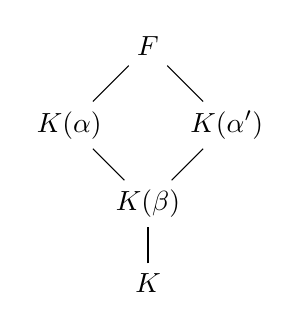
\begin{tikzpicture}
                \path (0, 0) node(K) {$K$} (0, 1) node (Kb) {$K(\beta)$} (-1, 2) node(Ka) {$K(\alpha)$} (1, 2) node(Kaa) {$K(\alpha')$} (0, 3) node(F) {$F$};
  
                \draw (K) -- (Kb);
  \draw (Kb) -- (Ka) -- (F);
  \draw (Kb) -- (Kaa) -- (F);
\end{tikzpicture}
        \end{figure}
        
        As $\beta$ is not in $K$, $[K(\beta) : K] = 2$ - the goal is to show that the degrees of $[K(\alpha) : K(\beta)] = [K(\alpha') : K(\beta) ] = 2$ and $[F : K(\alpha)] = [F : K(\alpha')] = 2$, and so by the tower law to arrive at $[F : K] = 8$.

Suppose $\alpha \in K(\beta) = \{ x + y\beta | x, y \in K \}$. So $\exists x, y \in K$ such that $\alpha = x + y\beta$. Then by the identity above
\[(x + y\beta)^2 = (x^2 + y^2b) + 2xy\beta = a + \beta\]
And
\[(x - y\beta)^2 = (x^2 + y^2b) - 2xy\beta = a - \beta\]
So
\[((x + y\beta)(x - y\beta))^2 = (a + \beta)(a - \beta) = a^2 - b = c\]
But
\[((x + y\beta)(x - y\beta))^2 = (x^2 - y^2b)^2\]
so $x^2 + y^2b \in K$, and $c$ is a square in $K$, which is a contradiction of the initial assumptions. So $\alpha \not \in K(\beta)$ - and a similar argument gives that $\alpha' \not \in K(\beta)$. So $[K(\alpha) : K(\beta)] = [K(\alpha') : K(\beta)] = 2$.

We also wish to show that $K(\alpha) \ne K(\alpha')$ - otherwise $F = K(\alpha) = K(\alpha')$. However -
\[(\alpha\alpha')^2 = (a + \beta)(a - \beta) = a^2 - b = c\]
So if $c$ is a square in $K$, then $\exists \gamma \in K$ with $\gamma^2 = c$, then $\alpha\alpha' = \pm\gamma \in K$ - so $K(\alpha) = K(\alpha')$.
        
        \begin{lem}
            Suppose $A$ is not a square in $F$, and $B \in F$. If $B$ is square in $F(\sqrt{A})$ then either $B$ is already a square in $F$, or $AB$ is a square in $F$.
        \end{lem}
        
        \begin{proof}
            We have that $B = (x + y\sqrt{A})^2 = x^2 + Ay^2 + 2xy\sqrt{A}$. But since $B \in F$, either $x, y = 0$. If $y = 0$, then $B$ is a square in $F$. If $x = 0$, then $B = y^2A$, so $BA = y^2A^2 = (yA)^2$ is a square in $F$.
        \end{proof}
        
        Suppose for a contradiction $\alpha' \in K(\alpha)$ - i.e. $a - \sqrt{b}$ is a square in $K(\alpha) = K(\beta)\sqrt{a + \sqrt{b}}$. Applying the lemma with $F = K(\beta)$, $A = a + \sqrt{b}$, $B = a - \sqrt{b}$. Then either $B$ is square in $F$, which is a contradiction, or $AB$ is square in $F$, i.e. $AB = a^2 -b = c$ is a square in $K(\beta)$. Apply the lemma again with $F = K$, $A = b$ and $B = c$. Then either $c$ is a square in $K$, which is a contradiction or $bc$ is a square in $K$, which is a contradiction. So $\alpha' \not \in K(\alpha)$.
        
        So $[L : K] = 8$, and $|G| = 8$.
        
        Now we want $G = D_8$.
        
        Let $\sigma \in G$. We have $\sigma(\beta) = \pm \beta$.
        
        If $\sigma(\beta) = \beta$ then $\sigma(\alpha) = \pm\alpha$ and $\sigma(\alpha') = \pm \alpha'$. 
        
        If $\sigma(\beta) = -\beta$ then $\sigma(\alpha) = \pm \alpha'$ and $\sigma(\alpha') = \pm \alpha$.
        
        But since $|G| = 8$, and there are 8 total permutations, all of these permutations are elements of $G$. These permutations are symmetries of a square with $\alpha, \alpha', -\alpha, -\alpha'$, so $G = D_8$. Let $\tau$ be the reflection that sends $\alpha' \mapsto -\alpha'$, and $\sigma$ the rotation that sends $\alpha \mapsto \alpha'$.
        
        We can find the subfields from the different combinations of symmetries, and what they fix. See appendix.
        
        
        
        \item Suppose that $bc$ is a square in $K$, but $c$ is not a square in $K$.
        
        Let $\gamma = \sqrt{c}$. Then $K(\beta\gamma) = K(\sqrt{bc}) = K$, and $K(\beta) = K(\gamma)$, so $K(\sqrt{b}) = K(\sqrt{c})$. We claim that $[L : K(\gamma)] = 2$, and $L = K(\alpha) = K(\alpha')$: indeed, suppose that $a + \beta$ is a square in $K(\beta)$. Then $\exists x,y \in K$ such that $(x + y\beta)^2 = a + \beta$, so $x^2 + y^2b + 2xy\beta = a + \beta$, then $x^2 + y^2b - 2xy\beta = a - \beta$. Then $(x^2 - by^2)^2 = ((x+ y\beta)(x-y\beta))^2 = (a + \beta)(a - \beta) = a^2-b = c$, so $c = (x^2 + y^2b)^2$ and is hence a square in $K$, which is a contradiction.
        
        Now we have the degree of $[L : K] = 4$, as $[L : K(\beta)] = 2$ and $[K(\beta) : K] =2$. Now we need to show that $G = C_4$.
        
        Take $\sigma \in G$. Then we have that same cases as before:
        \begin{itemize}
            \item $\sigma(\beta) = \pm \beta$
            \item If $\sigma(\beta) = \beta$ then $\sigma(\alpha) = \pm\alpha$ and $\sigma(\alpha') = \pm \alpha'$
            \item If $\sigma(\beta) = -\beta$ then $\sigma(\alpha) = \pm \alpha'$ and $\sigma(\alpha') = \pm \alpha$
        \end{itemize}
        
        But we can't have all 8 cases as before since $|G| = [L : K] = 4$, so what has changed?
        
        We know that $\alpha \alpha' = \gamma$, and $\beta \gamma \in K$, hence $\beta \gamma$ is fixed, so if $\sigma(\beta) = \beta$ then $\sigma (\gamma)$ depends on $\beta$. $\gamma'$ also depends on $\beta$. So actually $\sigma(\alpha)$ depends on where $\beta$ gets sent, and can only differ by where $\sigma(\alpha')$ gets sent (since $\alpha \alpha' = \gamma$), hence we can only have $2^2 = 4$ different $\sigma$.
        
        We also can choose $\sigma(\beta) = -\beta$ as the generator: it generates all $\sigma \in G$, hence $G = C_4$.
        

        
        \item Suppose $c$ is a square in $K$, but $bc$ is not a square - hence $\gamma = \sqrt{c} \in K$.
        
        We have $g(Y) = (Y^2 -2a -2\gamma)(Y^2 - 2a + 2\gamma)$, and $L$ is the splitting field of $g(Y)$, so it is worth thinking about $\delta, \delta'$ instead of $\alpha, \alpha'$. Then $[K(\beta) : K] = 2$, and $[K(\delta) : K] \le 2$ and $[K(\delta') : K] \le 2$.
        \begin{figure}[h]
            \centering
        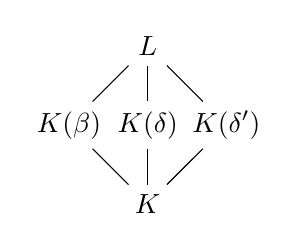
\begin{tikzpicture}
        \path (0, 0) node(K) {$K$} (-1, 1) node (Kb) {$K(\beta)$} (0, 1) node(Ka) {$K(\delta)$} (1, 1) node(Kaa) {$K(\delta')$} (0, 2) node(F) {$L$};
  
        \draw (K) -- (Kb) -- (F);
        \draw (K) -- (Ka) -- (F);
        \draw (K) -- (Kaa) -- (F);
        \end{tikzpicture}
        \end{figure}
        
        If $[L : K] = 4$, then $G = C_2 \times C_2$. Can $[L : K] = 2$?
        
        What about whether $2(a + \gamma)$, $2(a - \gamma)$ are squares in $K$? Suppose $2(a - \gamma)$ is not square in $K$. Can $2(a + \gamma)$ be a square in $K(\delta')$? By the lemma, we either have that $2(a + \gamma)$ is a square in $K$, or $2(a - \gamma)2(a + \gamma) = 4b$ is a square in $K$, which cannot happen as $b$ is not a square in $K$.
        
        Therefore either $[L : K] = 4$ and $G = C_2 \times C_2$, with $f(X)$ irreducible.
        
        Or ONE of $2(a \pm \gamma)$ is a square in $K$, $[L : K] = 2$ and $G = C_2$, with $f(X)$ NOT irreducible: $f(X) = X^4 - 2aX^2 + c = (X^2 - \delta X + \gamma)(X^2 + \delta X + \gamma)$, or switch for $\delta'$, whatever is actually an element of $K$ by $\sqrt{2(a \pm \gamma)} = \delta$ or $\delta'$.
    \end{enumerate}
    
    \begin{exmp}
        Look at $\sqrt{5 \pm 2\sqrt{6}}$. Then $f(X) = X^4 -10X^2 + 1$ and $c = 1$ which is a square, $b = 6$ is not a square, $\gamma = 1$ is a square - so we are in the last case. Then $2(a + \gamma) = 12$, $2(a - \gamma) = 8$, neither of which are a square, so $G = C_2 \times C_2$ hence $L = \Q(\sqrt{2}, \sqrt{3})$. Note, Galois theory explains why you have identities like $(\sqrt{2} + \sqrt{3})^2 = 5 + 2\sqrt{6}$.
    \end{exmp}
    
    \begin{exmp}
        Take $\sqrt{3 + 2\sqrt{2}}$. $f(X) = X^4 - 6X^2 + 1$. Then $a = 3$, $c = 1$, $b = 2$, $\gamma = 1$. So $c$ is a square, and $2(a + \gamma) = 8$ but $2(a - \gamma) = 4$ which is a square, so $[L : K] = 2$ and $G = C_2$.
    \end{exmp}
\end{proof}

\section{Finite fields}

If $F$ is finite, then it has $ch(F) = p >0$ for some prime $p$. Then $\mathbb{F}_p \subset F$. Because $F$ is finite, it is a finite dimensional vector space over $\mathbb{F}_p$.

As a vector space, $F \cong (\mathbb{F}_p)^m$, where $m = [F : \mathbb{F}_p]$, hence $|F| = |(\mathbb{F}_p)^m| = p^m$.

\begin{thm}
    Fix a prime $p > 0$. Then $\forall m \ge 1, m \in \Z$ then $\exists$ a unique (up to isomorphism) finite field with $q = p^m$ elements.
    
    We call this field $\mathbb{F}_q$.
\end{thm}

\begin{proof}
    Suppose $|F| = q = p^m$. We will prove that $F$ is unique. Then $F^X = F \setminus \{0\}$ is a group with $q-1$ elements - i.e. if $\lambda \in F \setminus \{0\}$ then $\lambda^{q-1} = 1$.
    \[X^{q-1} - 1 = \prod_{\lambda \in F^X}(X - \lambda) \in \mathbb{F}_p[X]\]
    Every such field is a splitting field of $X^{q-1} - 1$ for $\mathbb{F}_p$ - and any two splitting fields are isomorphic.
    
    For existence of $F$, let $F$ be the splitting field over $\F_p$ of $f(X) = X^{q-1} - 1 \in \mathbb{F}_p$. Let's try to prove it has $q$ elements.
    
    We have proved that $\F_p$ is a perfect field - so $\forall \lambda \in \F_p$, $\exists \mu \in \F_p$ such that $\lambda = \mu^p$. In particular, since every polynomial in $\F_p$ is separable, $f(X)$ has $q-1$ distinct roots in $F$.
    
    The claim is that $F' = \{0, \lambda, \lambda_1, ..., \lambda_{q-1}\}$ is a field (then clearly $F= F'$). So we want to show that $F'$ is closed under addition, multiplication and $F' \setminus \{0\}$ has multiplicative inverses.
    \begin{itemize}
        \item Closed under multiplication and inverses:
        
        $\{\lambda \; | \; \lambda^n = 1\}$ is a group (i.e. the $n$th roots of unity), so we have multiplicative inverses and it is closed under multiplication.
        
        \item Closed under addition:
        
        $\forall a,b \in F$ we know that $(a + b)^q = a^q + b^q$. 
    \end{itemize}
\end{proof}

\begin{rem}
    The Galois group $G = Gal(\F_q / \F_p) = \Z / m\Z$ is the cyclic group of order $m$. The function $F : \F_q \to \F_q$ which sends $a \mapsto a^p$ is a field automorphism of order exactly $m$ i.e. $F \in G$.
    
    It is clearly a field automorphism since $F(ab) = (ab)^p = a^pb^p = F(a)F(b)$, similar for $F(\frac{a}{b})$, and $F(a+b) = (a+b)^p = a^p + b^p = F(a) + F(b)$ (trivially, $F(1) = 1$ and $F(0) = 0$). It has order exactly $m$. Certainly, $F^m = id$ as $\lambda^{q-1} = 1$, so $\lambda^q = \lambda$. But if it had order of less than $m$, say $k$, then $\forall \lambda \in \F_q$, we have $\lambda^{p^k} = \lambda$, therefore $X^{p^k} - X$ has $q > p^k$ distinct roots, which is not possible.
\end{rem}

\section{Cubic Polynomials}

\[f(X) = X^3 - \sigma_1X^2 + \sigma_2X - \sigma_3\]

\subsection{Elemntary Symmetric Polynomials}

Consider
\begin{align*}
    f(x) &= (x- x_1)(x- x_2) ... (x- x_n) \\
         &= x^n -\sigma_1x^{n-1} + \sigma_2x^{n-2} ... \pm \sigma_n
\end{align*}
Where
\begin{align*}
    \sigma_1 &= \sigma_1(x_1, ..., x_n) = \sum_{1 \le i \le n} x_i \\
    \sigma_2 &= \sigma_2(x_1, ..., x_n) = \sum_{1 \le i < j \le n} x_i x_j \\
    ... \\
    \sigma_n &= \sigma_n(x_1, ..., x_n) = x_1 x_2 ... x_n
\end{align*}

We say that $\sigma_i \in K[x_1, ..., x_n]$ are the elementary, symmetric polynomials.

\begin{defn}
    A polynomial $\sigma \in K[x_1, ..., x_n]$ is symmetric if and only if $\forall g \in \mathfrak{S}_m$ a permutation, $\sigma(X_{g(1)}, X_{g(2)}, ..., X_{g(n)}) = \sigma(X_1, X_2, .., X_n)$. 
    
    I.e. it doesn't matter what permutation of variables you have, the equation is always equivalent.
\end{defn}

\begin{exmp}
    Consider $(X - X_1)(X - X_2) = X^2 - \sigma_1 X + \sigma_2$. Then $\sigma_i$ is a symmetric polynomial.
\end{exmp}

\begin{exmp}
    $\delta(x_1, x_2) = (x_1 - x_2)$ is not symmetric, but $\delta^2(x_1, x_2) = (x_1 - x_2)^2$ is symmetric.
    
    $\delta^2(x_1, x_2) = (x_1 - x_2)^2 = (x_1 + x_2)^2 - 4x_1x_2 = \sigma_1^2 - 4\sigma_2$ is the discriminant of the quadratic - doesn't depend on the order of the roots, just the sum and the product i.e. the coefficients of the polynomials. It is an invariant.
\end{exmp}

\subsection{Cubic invariant}

The goal is to find an invariant telling us when a cubic has repeated roots, like the discriminant of a quadratic polynomial.

We can use the $\delta$ function, which is 0 when there is a repeated root:
\[\delta(x_1, x_2, x_3) = (x_1 - x_2)(x_1 - x_3)(x_2 - x_3)\]
However, this not symmetric and so not invariant under the permutation group $\mathfrak{S}_3$, but it is invariant under the symmetric group $\langle (1 2 3) \rangle$.

$\delta^2 = \triangle$ is invariant, can we write it as a polynomial in $\sigma_1 = x_1 + x_2 + x_3$, $\sigma_2 = x_1x_2 + x_1x_3 + x_2x_3$ and $\sigma_3 = x_1x_2x_3$?

Yes - you can write it:
\[\triangle = \sigma_1^2\sigma_2^2 - 4\sigma_1^3\sigma_3 - 4\sigma_2^3 + 18\sigma_1\sigma_2\sigma_3 - 27\sigma_3^2\]

\begin{exmp}
    $x^3 + 3px + 2q$ has discriminant $\triangle = -2^23^3$ 
\end{exmp}

\subsection{Degree $n$ discriminant}

Questions:
\begin{enumerate}
    \item Can we find a formula for the discriminant of a degree $n$ polynomial?
    \item Is it a general fact that all symmetric polynomials are polynomials in the elementary symmetric polynomials.
\end{enumerate}


\begin{thm}
    Consider a degree $n$ separable polynomial
\[f(x) = x^n + a_1 x^{n-1} + ... + a_n \in k[X]\]
Let $k \subset L$ be the splitting field. Then the Galois group $G$ is contained in the alternating group $A_n$ if and only if $\triangle = \prod_{\text{roots of }f}(\lambda_i - \lambda_j)^2$ is a square in $k$
\end{thm}

\begin{proof}
    $G \subset A_n$ if and only if $\delta = \prod (\lambda_i - \lambda_j)$ is $G$-invariant if and only if $\delta \in k$. By the fundamental theorem of Galois theory, $\triangle \in k$ since $\triangle$ is symmetric i.e. $\mathfrak{S}_n$ invariant. By Galois theory, $k[x_1, ..., x_n]\mathfrak{S}_n \subset k(\sigma_1, ..., \sigma_n)$, and hence $\triangle$ is $G$-invariant and hence in $k$.
\end{proof}

\begin{rem}
    We know that in general, if $k \subset L$ is normal and separable ($L$ is the splitting field of $f \in k[x]$), then $G \subset \{\text{permutations of the roots of }f\}$.

If in addition, $f \in k[x]$ is irreducible, then $G$ is transitive i.e. given any $\lambda_1, \lambda_2$ roots of $f$, there exists $\sigma \in G$ such that $\sigma(\lambda_1) = \lambda_2$.
\end{rem}

\begin{proof}
    $k \subset k(\lambda_1) \subset L$ and $k \subset k(\lambda_2) \subset L$, hence $\sigma_0 : k(\lambda_1) \to k(\lambda_2)$ such that $\sigma_0(\lambda_1) = \lambda_2$.
\end{proof}

\subsection{Galois Group of Cubic Polynomial}

\begin{thm}
    Consider an irreducible polynomial cubic polynomial
    \[x^3 - \sigma_1 x^2 + \sigma_2 x - \sigma_3\]
    and let $k \subset L$ be the splitting field of the polynomial. Then
    \begin{itemize}
        \item $G = S_3$ if and only if $\triangle$ is not a square in $k$
        \item $G = A_3 = C_3$ if and only if $\triangle$ is a square in $k$
    \end{itemize}
\end{thm}

\section{Testing polynomials for irreducibility}

All polynomials here will be in $\Q[X]$ or $\F_p[X]$.

\subsection{Various Criterion}

\begin{prop}
    Suppose that a polynomial $f(x) = a_0 + a_1x + ... + a_d x^d \in \Z[X]$ has a rational root $\frac{p}{q} \in \Q$, $p,q$ coprime. Then $p | a_0$ and $q | a_d$.
\end{prop}

\begin{exmp}
    $f(x) = x^5 - 5$ has no rational roots. Note that this does NOT show that this polynomial is irreducible over $\Q$.
\end{exmp}

\begin{exmp}
    $f(x) = x^3 - 2$ has no rational roots and is irreducible (as any cubic with no rational roots is irreducible).
\end{exmp}

\begin{proof}
    $f(\frac{p}{q}) = a_0 + a_1 \frac{p}{q} + ... + a_d \frac{p^d}{q^d} = 0$. Now multiply by $q^d$:
    \[a_0q^d + a_1pq^{d-1} + ... + a_d p^d = 0\]
    Now $q \; |\; (a_0q^d + a_1pq^{d-1} + ... + a_{d-1}p^{d-1}q)$, and $q | 0$ trivially, so $q | a_d$ as $p, q$ are coprime.
    
    Similarly, $p \; | \; (a_1pq^{d-1} + ... + a_dp^d)$, so $p | a_0$.
\end{proof}

\begin{rem}
    If $K$ is a field, then $K[X]$ is a Euclidean domain, in particular unique factorisation holds. This also implies that $K[X]$ is an integral domain - i.e $\forall a,b \in K[X]$ if $ab = 0$ then either $a = 0$ or $b = 0$.
\end{rem}

Suppose that you want to show $n \in \Z$ is prime.
\begin{itemize}
    \item You can try to divide by all primes $p < \sqrt{n}$. For example, take $97$. Then you need to check all primes less than 10 - $2 \not | \; 97$, $3 \not | \; 97$, $5 \not | \; 97$, $7 \not | \; 97$ so we are done and it is prime.
\end{itemize}

Can such a method work with polynomials in $\Q[X]$?

Take $f(x) \in \Q[X]$ - can we check finitely many irreducible polynomials for division?
\begin{itemize}
    \item Yes, but we won't go there because it is not very practical by hand - there are many more things to check than with the integers.
\end{itemize}

This method is OK in $\F_p[X]$ - there are only finitely many coefficients to worry about for each particular degree.

This leads to a useful strategy:

\begin{exmp}
    Consider $x^5 - 5 \in \Q[X]$.
    \begin{itemize}
        \item Is it irreducible as a polynomial in $\F_2[X]$?
        
        $x^5 - 5 \equiv x^5 + 1 \pmod 2$, which has the root 1, so it is not irreducible.
        \item Is is irreducible in $\F_3[X]$?
        
        $x^5 - 5 \equiv x^5 + 1 \pmod 3$, which has the root -1, so it is not irreducible.
        \item Is it irreducible in $\F_5[X]$?
        
        No, trivially as $x^5-5 \equiv x^5 \pmod 5$.
        \item Is it irreducible in $\F_7[X]$?
        
        We would have to enumerate all the linear and quadratic irreducibles in $\F_7[X]$.
    \end{itemize}
\end{exmp}

\begin{lem}[Gauss' Lemma]
    Suppose $f(x) \in \Z[X]$, where the coefficients are coprime, factors non-trivially in $\Q[X]$. Then it factors non-trivially in $\Z[X]$.
\end{lem}

\begin{proof}
    Suppose $f(x) = g(x) h(x)$ in $\Q[X]$. $g(x), h(x) \in \Q[X]$. There is $c \in \Z$ such that $cf(x) = g'(x)h'(x)$ with $g'(x), h'(x) \in \Z[X]$ (taking the lowest common multiple of the denominators). We also have $g' = \lambda g$, $h' = \mu h$ where $\lambda, \mu \in \Q$. There is a smallest such $c \in \Z$. The claim is that $c = 1$.
    
    If $c \ne 1$, then there exists $p \in \Z$ prime that divides $c$. Take $cf(x) = g'(x) h' (x)$ modulo $p$:
    \[0 \equiv \overline{g'}(x) \overline{h'}(x) \in \F_p[X]\]
    But $\F_p[X]$ is an integral domain, so either $p | g'(x)$ hence it divides all of its coefficients, or $p | h'(x)$. But if $p$ divides all the coefficients of $g'(x)$, then we could reduce $cf(x) = g'(x)h'(x)$ by $p$ on both sides, and hence $c$ is not the smallest, which is a contradiction.
\end{proof}

\begin{cor}
    If $f(x)$ is prime in $\F_p[X]$, then it is prime in $\Q[X]$.
\end{cor}

\begin{proof}
    If a polynomial factors in $\Z[X]$, it factors in $\F_p[X]$, so taking the contrapositive, we obtain the corollary.
\end{proof}

So for our original example, as soon as we find out $x^5 - 5$ is irreducible in a prime field, we know it is irreducible in $\Q[X]$.

\begin{cor}[Eisenstein criterion]
    $f(x) = a_0 + a_1 x + ... + a_d x^d \in \Z[X]$ is irreducible if $\exists p$ prime such that $p \not | \; a_d$, but $p | a_i$ for $i < d$ and $p^2 \not | \; a_0$.
\end{cor}

\begin{proof}
    Work modulo $p$. Then $f(x) \equiv a_d x^d \pmod p$. If $f(x) = g(x)h(x)$ in $\Z[X]$ then $h(x) \equiv b_kx^k \pmod p$, $g(x) \equiv c_{d-k} x^{d-k} \pmod p$. That means that $h(x) \equiv b_0 + b_1 x + ... + b_k x^k$, $g(x) = c_0 + c_1 x + ... + c_{d-k}x^{d-k}$, where $p \; | \; b_i$ and $p \; | \; c_i$. Then $p^2 | a_0$ because $a_0  = c_0b_0$.
\end{proof}

Hence, $x^5 - 5$ is irreducible by this criterion - take $p = 5$, then $p \; | -5$, $p \not | \; 1$ and $p^2 \not | \; -5$.

\section{Cycle Type Theorem}

\subsection{Theorem and Examples}

\begin{thm}
    Let $f(x) \in \Z[X]$ be monic. Take $\Q \subset K$ be the splitting field of $f$ and $G \subset S_n$ ($G$ is a subset of the permutations of $K$) the Galois group.
    
    For $p$ prime, denote $f_p$ as the polynomial $f \in \mathbb{F}_p[X]$ (modulo the coefficients $p$). If $\exists p$ such that $f_p \in \mathbb{F}_p[X]$ is
    \begin{itemize}
        \item separable ($n$ distinct roots in any splitting field)
        \item $f_p = \prod_{i=1}^k \phi_i (x) \in \mathbb{F}_p[X]$ with $\phi_i$ of degree $n_i$ irreducible
    \end{itemize}
    then $\sigma \in G$ has a cycle type $(n_1)(n_2)...(n_k)$.
\end{thm}

Look up $spec \;\Z$ for motivation - maps $f$ to $f_p$ (for all primes $p$) as a topology.


\begin{exmp}
    We can use this theorem to write down an explicit degree 5 polynomial $f \in \Z[X]$ such that $G = S_5$ (the whole symmetric group).
    
    \begin{prop}
        Suppose that $r$ is prime. Let $G \subset S_r$ a subgroup of the symmetric group of size $r$. If $G$ contains an $r$-cycle, and 1 transposition, then $G = S_r$.
    \end{prop}
    
    \begin{proof}[Proof sketch for $r = 5$]
        Suppose that $(1,2,3,4,5) \in G$, and $(1,2) \in G$ - we can assume the transposition is $(1,2)$, since if we have $(1, x)$, then $\exists y$ such that $(1,2,3,4,5)^y = (1,x, ...)$ since $r$ is prime.
        
        Let $\sigma = (1,2,3,4,5)$. Then $\sigma^{-i}(1,2)\sigma^i = (i, i+1)$. This implies that $(1,2), (2,3), (3,4), (4,5) \in G$. A general fact, however, is that $\forall n$
        \[\langle (1,2), (2,3), ..., (n-1, n) \rangle = S_n\]
        Indeed, for any $a < b$, we have that $(a,b) = (a, a+1)(a+1,b)(a, a+1)$, so we can use this definition inductively to make $(a,b)$ out of consecutive 2-cycles. Any $\sigma \in S_n$ is a product of 2-cycles, hence we are done.
    \end{proof}
    
    The plan is:
    \begin{enumerate}
        \item find an irreducible, monic, degree 5 polynomial $\phi(x) \in \mathbb{F}_2[X]$
        \item find an irreducible, monic, degree 2 polynomial $\psi(x) \in \mathbb{F}_3[X]$
        \item find $f \in \Z[X]$ monic such that \[f \equiv \phi \in \mathbb{F}_2[X]\] and \[f \equiv x(x-1)(x+1)\psi \in \mathbb{F}_3[X]\] 
    \end{enumerate}
    The theorem implies that $G = S_5$.
    
    The irreducible polynomials of degree 2 are
    \begin{itemize}
        \item $x^2 + x + 1 \in \mathbb{F}_2[X]$
        \item $x^2 + 1 \in \mathbb{F}_3[X]$
    \end{itemize}
    The claim is that
    \[\phi(x) = x^5 + x^3 + 1 \in \mathbb{F}_2[X]\]
    is irreducible. Indeed, it has no linear factor as it has no roots, and it is not divisible by $x^2 + x + 1$ - the only irreducible of degree 2.
    
    Now let $\psi(x) = x^2 + 1$:
    \[x(x-1)(x+1)(x^2 + 1) = x^5 - x\]
    
    We can now find $f \in \Z[X]$ using the Chinese Remainder Theorem (and common sense/intuition, seriously you've done this a million times before)
    \[f(x) = x^5 +3x^2 +2x + 3 \in \Z[X]\]
\end{exmp}

To prove the original theorem, we need some other theorems.

\subsection{Helper Theorems}

\begin{prop}
    Let $f(x) \in \F_p[X]$ be a polynomial. Let $\{\lambda_i\}$ be the roots of $f$. Then $\F_p(\lambda_i)$ is the whole splitting field of the polynomial (i.e. contains all the other roots as well).
    
    Take any 2 splitting fields of $f$, $K$ and $K'$. Then $K = K'$.
    
    Let $f, f' \in \F_p[X]$ have the same degree. Let $K$ be the splitting field for $f$, $K'$ the splitting field for $f'$. Then $K = K'$.
\end{prop}

\begin{defn}[Monoid]
    A monoid is a structure that is made up of a set of elements and an operation that is
    \begin{enumerate}
        \item associative
        \item commutative
        \item NOT invertible
    \end{enumerate}
    It is usually denoted $P$.
\end{defn}

\begin{defn}[Character]
    A character from a monid $P$ to a field $K$ is a function $\chi$ such that
    \[\chi(0) = 1\]
    \[\chi(p_1 + p_2) = \chi(p_1)\chi(p_2)\]
    for $p_1, p_2 \in P$.
\end{defn}

\begin{thm}[Dedekind Independence Theorem]
    Let $K$ be a field, $P$ a monoid (an algebraic structure with an operation that is commutative, associative, but NO inverses). Then any set of distinct characters
    \[\chi_1 : P \to K\]
    \[\chi_2 : P \to K\]
    \[...\]
    \[\chi_n : P \to K\]
    is linearly independent in the vector space
    \[\{f : P \to K\}\]
\end{thm}

\begin{rem}
    If $K$ is a field and $A$ a set then
    \[\{f : A \to K\}\]
    is a $K$-vector space.
\end{rem}

\begin{proof}
    Assume for a contradiction that $chi_i$ are linearly independent:
    \[ (\dagger) \; \lambda_1 \chi_1 + ... \lambda_n \chi_n = 0 \]
    with $\lambda_i \in K$. We may assume that $n$ is the smallest such that for this statement, hence $\forall i$, $\lambda_1 \ne 0$. For $n \ge 2$, $\exists p$ such that $\chi_1(p) \ne \chi_2(p)$. Hence
    \[\lambda_1 \chi_1(p) \chi_1 + ... \lambda_n \chi_n(p) \chi_n = 0\]
    so this is a multiple of $(\dagger)$ from our initial assumption of $(\dagger)$ being the shortest such statement. Hence $\chi_1(p) = \chi_2(p)$, so we have a contradiction.
\end{proof}

\begin{thm}
    Let $f(x) \in \Z[X]$ be a monic polynomial of degree $n$. Let $\Q \subset K$ be a splitting field for $f$. Say $f(x) = \prod_{i=1}^n (x-\lambda_i)$ with $\lambda_i \in K$.
    
    Let $p$ be a prime. Denote $\overline{f} \in \F_p[X]$ as taking "$f \mod p$". Let $\F_p \subset F$ be a splitting field for $\overline{f}$. Assume that $\overline{f}$ is separable.
    
    Let $R \subset K$ be the subring generated by the roots of $f$, i.e. $R = \Z[\lambda_1, ..., \lambda_i]$.
    
    Then
    \begin{enumerate}
        \item There exists a ring homomorphism $\psi : R \to F$.
        \item Any ring homomorphism $\psi' : R \to F$ induces a bijection $\psi' : Z \to Z_p$ where $Z = \{\lambda_1, ..., \lambda_n\}$ and $Z_p = \{\text{roots of } \overline{f}\}$.
        \item Say $\psi : R \to F$ is the ring homomorphism as from $(1)$. Then $\psi' : R \to F$ is a ring homorphism if and only if $\exists \sigma \in G$ such that $\psi' = \psi \circ \sigma$.
    \end{enumerate}
\end{thm}

\begin{proof}
    \begin{enumerate}
        \item $R$ is as finitely generated, free $\Z$-module - $R$ is generated as a $\Z$-module by $\{\lambda_1^{e_1}, ..., \lambda_n^{e_n}\}$ and since all $\lambda_i$ satisfy the polynomial $f$, we have $0 \le e_i < n$.
        \item Let $u_1, ..., u_d$ be a basis of $R$ as a $\Z$=module. Claim: then this is also a basis of $K$ as a $\Q$-vector space, hence $d = [K : \Q]$.
        
        $u_1, ..., u_d$ are clearly independent over $\Q$. Take $\Q R \subset K$. $\Q R \supset \Q$ is a subring, which implies that $\Q R$ is a subfield (if $K \subset L$ is a finite field extension, and $K \subset R \subset L$ with $R$ a ring, then $R$ is a field). But $\Q R$ contains all the roots of $f$, and since $K$ is the smallest splitting field, we have $\Q R = K$. Therefore, $u_1, ..., u_d$ generate $K$ over $\Q$.
        \item Proof of $(1)$:
        \[\exists \psi : R \to F\]
        
        Let $\mathfrak{m} \supset \langle p \rangle$ be a maximal ideal in $R$. Then $\F_p \subset R / \mathfrak{m}$ is a finite field - $\mathfrak{m}$ contains $p$, so it contains all elements modulo $p$.
        \[\pi : R \to R / \mathfrak{m}\]
        \[f(x) =  \prod(x-\lambda_i) \in R[X]\]
        implies that
        \[\overline{f}(x) = \prod(x - \pi(\lambda_i)) \in R / \mathfrak{m}[X]\]
        Since $R$ is generated by $\lambda_i$, we have that $R / \mathfrak{m}$ is generated by $\pi(\lambda_i)$. This means that $R / \mathfrak{m}$ is a splitting field for $\overline{f} \in \F_p[X]$. But since all finite fields of a degree are isomporphic, this means that $R / \mathfrak{m} \cong F$ as the homomorphism is $pi = \psi$.
        \item Proof of $(2)$:
        
        Take
        \[\psi : R \to F\]
        Then the expression
        \[f(x) = \prod (x-\lambda_i)\]
        maps to
        \[\overline{f}(x) = \prod (x - \psi(\lambda_i))\]
        so the set of roots $\lambda_i$ maps to the set of $\psi(\lambda_i)$ which are all distinct, so there's a bijection.
    \end{enumerate}
\end{proof}





















\appendix

\section{}

% \begin{tikzpicture}
%   \path (0, 0) node(K) {$K$} (-1, 1) node (Kb) {$K(\beta)$} (0, 1) node(Kbg) {$K(\beta \gamma)$} (1, 1) node(Kg) {$K(\alpha')$} (0, ) node(Ka) {$K(\alpha)$} () node(Ka') {$$} () node(Kb,g) {} () node(Kd) {} () node(Kd') {} () node(L) {$L$};
  
%   \draw (K) -- (Kb);
%   \draw (Kb) -- (Ka) -- (F);
%   \draw (Kb) -- (Kaa) -- (F);
% \end{tikzpicture}

\section{Question 11, exmp. sheet 1}

Let $K$ be a field, and $ch(K) \ne 2$.

Let $F = K(\sqrt{a + \sqrt{b}}, \sqrt{a - \sqrt{b}})$, where $a,b \in K$, and $b$ is not a square in $K$.

Let $\alpha = \sqrt{a + \sqrt{b}}$. Then \[\alpha^2 = a + \sqrt{b}\] \[(\alpha^2 - a)^2 = b\] Hence \[\alpha^4 - 2a\alpha^2 +a^2 - b = 0\] so $\alpha$ is a root of $X^4 - 2aX^2 + c = 0$, where $c = a^2 - b$. Let \[f(x) = x^4 - 2ax^2 + c  \in K[X]\]

Note that $F$ is the splitting field of $f(x)$. Indeed, from the quadratic formula: $x^2 = a \pm \sqrt{b}$ so $x = \pm \sqrt{a \pm \sqrt{b}}$. So $K \subset F$ is a normal extension.

Let $\alpha' = \sqrt{a - \sqrt{b}}$, so $\pm \alpha$ and $\pm \alpha'$ are the roots of $f(x)$, and $F = K(\alpha, \alpha')$. We will see that if $ch(K) \ne 2$, then the extension is separable.

Right now, assume $f(x)$ is irreducible (we will see later a proof of this).

This implies that $b$ is not a square in $K$. Indeed, $f(x) = (x^2 - a -\sqrt{b})(x^2 - a + \sqrt{b})$.

Question: Study how $f(x) \in K[X]$ can be reducible in extensions of $K$.

Assuming $f(x)$ is irreducible, then we want to know:
\begin{enumerate}
    \item $[F : K] = ?$
    \item What is $G = Gal(F / K)?$ And what are all the subfields $K \subset L \subset F?$
\end{enumerate}

Answer:
If $c$ is a square in $K$
\begin{enumerate}
    \item $[F : K] = 4$
    \item $G \cong C_2 \times C_2$
\end{enumerate}
If $c$ is not a square in $K$, but $bc$ is a square
\begin{enumerate}
    \item $[F : K] = 4$
    \item $G \cong C_4$
\end{enumerate}
If neither $c$ nor $bc$ are squares in $K$
\begin{enumerate}
    \item $[F : K] = 8$
    \item $G \cong D_8$
\end{enumerate}

The actual question 11 on problem sheet 1 shows that if $b,c, bc$ are not squares, then $[F : K] = 8$.

\subsection{Working through the question}
Let $a, b \in K$ and set $c = a^2 - b$; suppose that none of $b$, $c$, or $bc$ is a square in $K$.
If $L$ is a splitting field of the polynomial:
\[(x^2 - a)^2 - b \in K[x]\]
prove that $[L : K] = 8$.

Let $\beta = \sqrt{b}$. Let $\alpha^2 = a + \beta$. Then

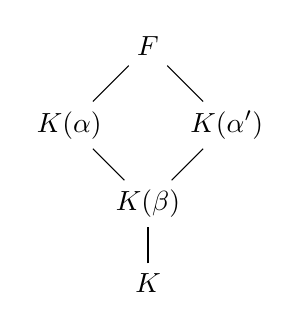
\begin{tikzpicture}
  \path (0, 0) node(K) {$K$} (0, 1) node (Kb) {$K(\beta)$} (-1, 2) node(Ka) {$K(\alpha)$} (1, 2) node(Kaa) {$K(\alpha')$} (0, 3) node(F) {$F$};
  
  \draw (K) -- (Kb);
  \draw (Kb) -- (Ka) -- (F);
  \draw (Kb) -- (Kaa) -- (F);
\end{tikzpicture}

As $\beta$ is not in $K$, $[K(\beta) : K] = 2$ - the goal is to show that the degrees of $[K(\alpha) : K(\beta)] = [K(\alpha') : K(\beta) ] = 2$ and $[F : K(\alpha)] = [F : K(\alpha')] = 2$, and so by the tower law to arrive at $[F : K] = 8$.

Suppose $\alpha \in K(\beta) = \{ x + y\beta | x, y \in K \}$. So $\exists x, y \in K$ such that $\alpha = x + y\beta$. Then by the identity above
\[(x + y\beta)^2 = (x^2 + y^2b) + 2xy\beta = a + \beta\]
And
\[(x - y\beta)^2 = (x^2 + y^2b) - 2xy\beta = a - \beta\]
So
\[((x + y\beta)(x - y\beta))^2 = (a + \beta)(a - \beta) = a^2 - b = c\]
But
\[((x + y\beta)(x - y\beta))^2 = (x^2 - y^2b)^2\]
so $x^2 + y^2b \in K$, and $c$ is a square in $K$, which is a contradiction of the initial assumptions. So $\alpha \not \in K(\beta)$ - and a similar argument gives that $\alpha' \not \in K(\beta)$. So $[K(\alpha) : K(\beta)] = [K(\alpha') : K(\beta)] = 2$.

We also wish to show that $K(\alpha) \ne K(\alpha')$ - otherwise $F = K(\alpha) = K(\alpha')$. However -
\[(\alpha\alpha')^2 = (a + \beta)(a - \beta) = a^2 - b = c\]
So if $c$ is a square in $K$, then $\exists \gamma \in K$ with $\gamma^2 = c$, then $\alpha\alpha' = \pm\gamma \in K$ - so $K(\alpha) = K(\alpha')$.

Suppose for a contradiction that $\alpha' \in K(\beta)(\alpha)$ i.e. that $a - \beta$ is square in $K(\beta)(\alpha)$.

Please read the solution sheet on Bea Corti's website :)

\end{document}
